%----------------------------------------------------------------------------
%	PACKAGES AND OTHER DOCUMENT CONFIGURATIONS
%-----------------------------------------------------------------------------
\RequirePackage[l2tabu, orthodox]{nag}
\documentclass[12pt]{article} % Default font size is 12pt
\usepackage[utf8]{inputenc} 
\usepackage[T1]{fontenc}
\usepackage[english]{babel} 
\usepackage[margin=2.5cm]{geometry}
\geometry{a4paper}
\usepackage{multirow}
\usepackage{longtable}
\usepackage{array,arydshln}
%\setlength\dashlinedash{0.2pt}
%\setlength\dashlinegap{4.5pt}
%\setlength\arrayrulewidth{0.2pt}
\newcolumntype{C}[1]{>{\centering\arraybackslash}m{#1}}
\newcolumntype{R}[1]{>{\raggedleft\arraybackslash}m{#1}}

\usepackage{multicol}
\usepackage{lscape}
\usepackage{soul} 
\usepackage{todonotes}
\usepackage{tabularx}



%----------------------------KODE START---------------------------------------
\usepackage{listings}
\usepackage{color}
\usepackage[usenames,dvipsnames]{xcolor}
\definecolor{gray}{rgb}{0.5,0.5,0.5}
\definecolor{mauve}{rgb}{0.58,0,0.82}
\lstset{
  basicstyle=\footnotesize,
  numbers=left,
  numberstyle=\tiny\color{gray},
  stepnumber=1,
  numbersep=8pt,
  backgroundcolor=\color{white},
  showspaces=false,               % show spaces adding particular underscores
  showstringspaces=false,         % underline spaces within strings
  showtabs=false,                 % show tabs within strings adding particular underscores
  frame=single,                   % adds a frame around the code
  rulecolor=\color{black},        
  tabsize=4,
  captionpos=b,                   % sets the caption-position to bottom
  breaklines=true,                % sets automatic line breaking
  breakatwhitespace=false,        % sets if automatic breaks should only happen at whitespace
  title=\lstname,                   % show the filename of files included with \lstinputlisting;
                                  % also try caption instead of title
  keywordstyle=\color{mauve},          % keyword style
  commentstyle=\color{Maroon},       % comment style
  stringstyle=\color{BlueViolet},         % string literal style
  escapeinside={\%*}{*)},            % if you want to add LaTeX within your code
  morekeywords={*,...},              % if you want to add more keywords to the set
  deletekeywords={...}              % if you want to delete keywords from the given language
}
%----------------------------KODE SLUT----------------------------------------

\setlength\parindent{0pt} % Makes \noindent standard for entire document
\usepackage{graphicx} % Required for including pictures
\usepackage[font={footnotesize},labelfont=bf]{caption}
\usepackage[font={footnotesize},labelfont=bf]{subcaption}
\usepackage{float} % Allows putting an [H] in \begin{figure} to specify the exact location of the figure
\usepackage{wrapfig} % Allows in-line images if needed
\usepackage{hyperref}
\usepackage{url}
\usepackage{cleveref}
\usepackage{amsmath}
\usepackage{mathtools}
\hypersetup{colorlinks=false,hidelinks, citecolor=black, urlcolor=black}
\usepackage{csquotes}
\usepackage{comment}

\usepackage[dot, autosize, outputdir="dotgraphs/"]{dot2texi}
\usepackage{booktabs}
\usepackage{multirow}
\usepackage{longtable}
\setcounter{secnumdepth}{4}
\setcounter{tocdepth}{4}
\usepackage[titletoc]{appendix} % Names appendices "Appendix A" instead of just A in Contents
\usepackage[bottom]{footmisc}
\usepackage{pdfpages}

\newcommand*{\rom}[1]{\expandafter\@slowromancap\romannumeral #1@}


%TIKZ STUFF STARTS

%\usetikzlibrary{arrows,positioning}
%\usetikzlibrary{arrows,automata}
%\usetikzlibrary{mindmap,trees}
\usepackage{tikz}
\usetikzlibrary{timeline}
%\usetikzlibrary{decorations.pathmorphing}
%\usetikzlibrary{shapes}

%TIKZ STUFF ENDS

\usepackage{verbatim}

\linespread{1.2} % Line spacing
\graphicspath{{./Pictures/}} % Specifies the directory where pictures are stored


% fancy drawings
\usepackage{pgf}
\usepackage{epigraph}

% \epigraphsize{\small}% Default
\setlength\epigraphwidth{8cm}
\setlength\epigraphrule{0pt}

\usepackage{etoolbox}
\usepackage{lmodern}


\makeatletter
\patchcmd{\epigraph}{\@epitext{#1}}{\itshape\@epitext{#1}}{}{}
\makeatother

%\usepackage{boxproof}
%\usepackage{nomencl}
\usepackage{natbib}

\newcommand{\fasto}{\textsc{Fasto} }
\newcommand{\mips}{\textsc{Mips} }
\newcommand{\mars}{Mars }

%-----------------------------------------------------------------------------
% HEADER AND FOOTER STUFF
%-----------------------------------------------------------------------------
\usepackage{fancyhdr}
\usepackage{lastpage} % Making it possible to write ``Page x of y'' in the footer

\pagestyle{fancy}
\fancyhf{}
% Header stuff below
\lhead{Jenny-Margrethe Vej} 
\chead{}
\rhead{rwj935} 
% Footer stuff below
\cfoot{Page \thepage \hspace{1pt} of \pageref{LastPage}} % To the left at the bottom

%-----------------------------------------------------------------------------
\begin{document}

\includepdf[pages={-}]{../forside_tex_ting/forside.pdf}

\begin{abstract} 
  
\end{abstract}

%Fra Torbens slide: 
%Et resumé (abstract) er
%En uhyre kort (5-20 linjer), præcis, kvantitativ beskrivelse af resultaterne i rapporten.
%Kun resultater! Metodik skal kun medtages, hvis den er relevant for at fortolke resultaterne. Alt andet er ligegyldigt
%Tænk: Hvis en meget travl beslutningstager (institutleder/direktøren/Torben) skal beslutte, om dokumentet er hans tid værd, skal vedkommende kunne afgøre det fra resuméet.
%Remember to make the abstract both in danish and english - english first\\

\newpage
\tableofcontents
%\nocite{*}

\newpage
\renewcommand{\abstractname}{Acknowledgements}
\begin{abstract}
\end{abstract}

\newpage  
\listoffigures
\addcontentsline{toc}{section}{List of Figures} %\caption[short caption for lof/lot]{long figure/table caption}

\listoftables
\addcontentsline{toc}{section}{List of Tables} %\caption[short caption for lof/lot]{long figure/table caption}

\newpage
\section{Introduction}
Explorative data, hypotheses is made after variables is found, I'm looking to find the variables 
\todo[inline]{write chapter (see notes from Kate)}

\newpage
\section{Related Work}
This chapter presents state of the art work in three areas and its current methods for quality and quantity assessment: sleep, wearables used for sleep monitoring and aspects on how smartphones can be used to assess sleep. This project is based on data collected from a smartphone application, but to understand the received data, and to be able to compare it with ground truth data from a wearable, it is important to have a basic understanding of sleep and wearables.

\subsection{Sleep}
This section is about sleep research in general. This project is focusing on healthy people. \\

All human beings are following a roughly 24-hour cycle called a circadian rhythm \cite{bewellSleep}. This rhythm is like the big body clock controlling all the small biological clocks in our body and includes not only our biological 24-hour circle but also regular changes in cortisol, hormones like melatonin, and blood pressure \cite{bewellSleep}. In 1960 biologist Curt Richter noted the circadian rhythm for the first time \cite{circadian}, and along years after, many studies were made on animals to research relations between activity, sleep, and this 24-hour clock. In 1965 Jürgen Aschoff, one of the pioneers in this kind of study, called chronobiology, wrote that \textit{``whatever physiological variables we measure, we usually find that there is a maximum value at one time of day and minimum value at another''} \cite{rhythm}. Aschoff was the first to study these rhythms in human beings. Aschoff also built a bunker to be able to isolate cues coming from timelike aspects \cite{rhythm2} and was able to prove the hypothesis that the human body clock is entrained by light. These findings created a new model stating that the circadian clock inside human beings uses external information to remain synchronised with environmental changes \cite{bewellSleep}.

\subsubsection{Definition of Sleep}
Sleep is a result of very complex interactions between several biochemical processes. We all have an internal battle between two mechanisms working against each other in the neural network responsible for sleep and wake activities. These are called the 'internal circadian oscillator' and 'the homeostatic system' - the first one is promoting wakefulness throughout the day, and the latter is increasing the drive to sleep the longer we have been awake \cite{promise}. When we go to sleep - the timing is determined by this circadian drive, and the duration is determined by the homeostatic system \cite{life}. A third factor, our social interactions such as social relationships and work, accompanies these two factors, giving people three highly complicated and individually diverse factors influencing and affecting our timing and quality of sleep: our circadian system, a homeostatic oscillator, and our social time.\\

A night of sleep consists of cycles of REM and NREM and the American Academy of Sleep Medicine (AASM) \cite{aasm} divides NREM into three stages: N1, N2, and N3, with the last stage, also called delta sleep or slow-wave sleep \cite{visual}. 

\subsubsection{Rapid-Eye-Movement (REM)}
\begin{wrapfigure}{r}{0.5\textwidth}
  \begin{center}
    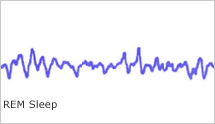
\includegraphics[width=0.48\textwidth]{img/rem}
  \end{center}
    \vspace{-20pt}
  \caption{EEG of a typical REM sleep \cite{harvard}.}
  \label{fig:rem}
\end{wrapfigure}

REM sleep is often called ``active sleep'' and measuring it with an EEG test it is typically identifiable by its low-amplitude, high-frequency waves, and alpha rhythm, as well as the eye movements it is named after \cite{harvard}. What is interesting is, that even though the eyes moves rapidly when in REM sleep, the muscles in arms and legs are paralysed, supposedly to prevent us from acting out the dreams, we have during this stage. In figure \ref{fig:rem} a typical REM sleep seen from an EEG monitor is shown. A typically healthy adult's sleep consists of around 20 to 25 percent REM sleep. 

\subsubsection{Non-Rapid-Eye-Movement (NREM)}
\begin{wrapfigure}{r}{0.5\textwidth}
  \vspace{-25pt}
  \begin{center}
    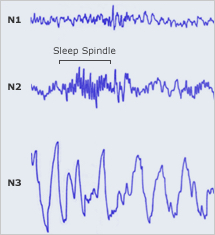
\includegraphics[width=0.48\textwidth]{img/nrem}
  \end{center}
    \vspace{-20pt}
  \caption{EEG of typical NREM sleep showing all three stages \cite{harvard}.}
        \vspace{-20pt}
  \label{fig:nrem}
\end{wrapfigure}

As the name indicates, NREM sleep is where the eyes are still. Going from stage N1 to N3 the brain waves becomes slower and more synchronised. Stage N3 is the deepest of the NREM stages, and is also referred to as ``deep'' or ``slow-wave'' sleep \cite{harvard}. As seen in figure \ref{fig:nrem} an EEG shows the high-amplitude, low-frequency waves, and spindles opposite to the REM sleep illustrated in figure \ref{fig:rem}. 


\subsubsection{The Night Sleep Cycle}
The cycling during a night's sleep between the four stages is in a healthy adult typically seen starting with NREM sleep. Stage N1 is the first stage of sleep and lasts only 1 to 7 minutes. The second stage is N2 which lasts around 10 to 25 minutes, and then the cycle moves on to stage N3 - the ``slow-wave'' sleep. 

\begin{wrapfigure}{r}{0.5\textwidth}
  \begin{center}
    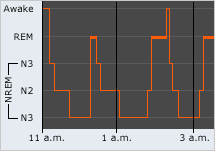
\includegraphics[width=0.48\textwidth]{img/hyp}
  \end{center}
    \vspace{-20pt}
  \caption{Hypnogram showing the typical patterns of REM and NREM sleep during a night \cite{harvard}.}
  \label{fig:hyp}
\end{wrapfigure}

This sleep stage generally lasts 20 to 40 minutes, and by now it becomes increasingly difficult to wake an individual from sleep \cite{harvard}. After the N3 stage, the body goes back to a short 5 to 10 minutes period in the N2 stage before continuing to a REM sleep episode. \\

The cycle continues during the night with more and more REM sleep and lesser N3 sleep illustrated in figure \ref{fig:hyp}. According to Harvard Medical School \cite{harvard} no scientists know the reason for this cycling pattern during the night. 

\subsubsection{Sleep Quantity Recommendations}
The National Sleep Foundation updated their recommendations on how much sleep a person needs in 2015 based on a literature study. They used the RAND/UCLA Appropriateness Method to define recommendations for sleep duration based on age \cite{duration}. Table \ref{tab:recommendation} shows a sample of the full table with recommendations on sleep periods from the National Sleep Foundation. 

\begin{table}[H]
\center
\begin{footnotesize}
	\begin{tabular}{|p{2.5cm} |p{3.3cm} |p{3.5cm} |p{3.5cm} |}
	\hline
	\textbf{Age} & \textbf{Recommended} & \textbf{May be appropriate} & \textbf{Not recommended} \\
	\hline
Teenagers & 8-10 & 7 or 11 & Less than 7\\
14-17 years & & & More than 11\\
	\hline
Young adults & 7-9 & 6 or 10-11 & Less than 6\\
18-25 years & & & More than 11\\
	\hline
Adults & 7-9 & 6 or 10 & Less than 6\\
26-64 years & & & More than 10\\
	\hline
Older adults & 7 to 8 & 5-6 or 9 & Less than 5\\
65 years or older & & & More than 9\\
	\hline
	\end{tabular}
	\caption{Recommendations on sleep duration for young people and adults made by the National Sleep Foundation \cite{duration}.}
	\label{tab:recommendation}
\end{footnotesize}
\end{table}

In 1982 the Cancer Prevention Study II (CPSII) collected more than 1.1 million questionnaires from American Adults ranging from 30 to 102 years of age. Six years later the survival rate was ascertained \cite{arch}. This study showed that sleeping between 6.5 and 7.4 hours each night, gave the best chances of survival. People who slept 6 hours or less and 8 hours or more had a significantly increased mortality rate. The study also showed that it was consistent gender and ages. \\

In 1984 University College London (UCL) started their Whitehall \rom{2} Study and based on data from phase 5 (1997-1999) and phase 7 (2003-2004) a study was made to see if and how changes in sleep duration affect a person's cognitive function. 5431 middleaged participants' data was used \cite{cognitive}. The results show the same trends as in Kripke et al. \cite{arch}. Increasing sleep duration from 7 or 8 hours of sleep results in a poorer cognitive function which is also the case if decreasing from 6, 7, or 8 hours of sleep. 

\subsubsection{Clinical Assessment of Sleep Quality}
In 2016 a comparison review was made on studies available with sleep as the focus area \cite{consumer}. Traditionally the `golden standard' for measuring sleep is polysomnography (PSG). Another device used in clinical sleep medicine is a wrist-worn devise called Actigraphy which is based on the principle that physical movements are increased when an individual are awake and reduced during sleep. According to B. P. Kolla et al. only a few studies have been made to compare data from wearable devices with PSG and actigraphy, and this review is based on those studies and is aimed at practicing clinicians \cite{consumer}. PSG and actigraphy typically measure the sleep parameters listed in Table \ref{tab:psgparameters}. 

\begin{table}[H]
\center
\begin{footnotesize}
	\begin{tabular}{|p{3.2cm} |p{4.6cm} |p{6.5cm} |}
	\hline
	\textbf{Parameter} & \textbf{Definition} & \textbf{Relevance}\\
	\hline
	Sleep latency (SL) & Time taken to fall asleep & Can be prolonged in patients with insomnia complaining of difficulty initiating sleep \\
	\hline
	Total Recording Time (TRT) & Time in bed until time out of bed & Total duration of recording\\
	\hline
	Wake After Sleep Onset (WASO) & Time spend awake after initially falling asleep & Can be prolonged in patients with insomnia complaining of difficulty maintaining sleep \\
	\hline
	Total Sleep Time (TST) & TRT - WASO & \\
	\hline
	Sleep efficiency (SE) & TST / TRT $\times$ 100 & Gives a measure on time spent asleep of total time in bed \\
	\hline
	Arousal index & Number of arousals / TST (arousal = wake period < 10 s) & Excess number of arousals and awakenings suggests increased sleep fragmentation\\ 
	\hline
	Awakening index & Number of arousals / TST (awakening = wake period > 10 s & Excess number of arousals and awakenings suggests increased sleep fragmentation \\
	\hline
	\end{tabular}
	\caption{Typical parameters measured with PSG and actigraphy as listed in \cite{consumer}}
	\label{tab:psgparameters}
\end{footnotesize}
\end{table}

\subsubsection{Sleep Quality Recommendations}
Going through literature, `sleep health' is a frequently used term but it is typically not defined. In 2014 Daniel J. Buysse was proposing a definition based on a positive attribute rather than a definition including any individual sleep disorder:
\textit{``Sleep health is a multidimensional pattern of sleep-wakefulness, adapted to individual, social, and environmental demands, that promotes physical and mental well-being. Good sleep health is characterised by subjective satisfaction, appropriate timing, adequate duration, high efficiency, and sustained alertness during waking hours.''} \cite{define}. 
The definition is builded on five dimensions of sleep; alertness, efficiency, duration, timing, and satisfaction. These dimensions are defined as appropriate because they can be expressed in positive terms, most of them can be measured by self-reporting and analysis of behavioral and psychological levels, and they all are understandable for both professionals and members of the public. \\

A generally accepted definition of `sleep quality' can be just as hard to find as a definition of `sleep health'. However, in 2012 Hamdan et al. used several sleep quality parameters for their study using biofeedback and ambient intelligence to monitor the quality of sleep \cite{Hamdan2012ABS}. In this study, they created a Total Sleep Index (TSI) that indicates the overall sleep quality. The parameters used to calculate their TSI is listed in Table \ref{tab:sleepQuality} along with optimal values for the parameters and how to measure them. The parameters are based on healthy people. 

\begin{table}[H]
\center
\begin{footnotesize}
	\begin{tabular}{|p{4cm} |p{2.6cm} |p{4cm} |p{3.3cm} |}
%	\begin{tabular}{| c | c | c | c |}
	\hline
	\textbf{Parameters} & \textbf{Optimal Value} & \textbf{Description} & \textbf{Sensors} \\
	\hline
	Sleep efficiency (SE) & $>$ 95\% & total sleep time $\times$ 100 / total time in bed & Electrocardiography, \newline Actimeter\\
	\hline
	Sleep latency (SL) & $<$ 15 minutes & Time from lights off till beginning of sleep & Electrocardiography, \newline Actimeter\\
	\hline 
	Number of awakenings (NA) & $<$ 10 & Number of awakenings during night & Electrocardiography, \newline Actimeter\\
	\hline
	Wake after sleep onset (WASO) & $<$ 15 minutes & The total time spent awake during sleep period time & Electrocardiography, \newline Actimeter\\
	\hline
	Periodic limb movements index (PLMI) & $<$ 30/h & Average number of limb movements per hour & Actimeter\\
	\hline
	Stage 1 percentage (S1) & 1-5\% of total sleep time & Stage 1 time / total sleep time & Electrocardiography\\
	\hline
	Stage 2 (light sleep) percentage (S2) & 50\% of total sleep time & Stage 1 time / total sleep time & Electrocardiography\\
	\hline
	Stage 3 and 4 (deep sleep) percentage (S34) & 10-20 \% of total sleep time & Stage 3 and 4 time / total sleep time & Electrocardiography\\
	\hline
	REM percentage (PR) & 20-25 \% of total sleep time & Stage REM time / total sleep time & Electrocardiography\\
	\hline
	REM latency (RL) & 90 minutes & Time from beginning of sleep until appearance of first REM sleep & Electrocardiography\\
	\hline
	Respiratory Disturbance Index (RDI) & $<$ 5/h & Average number of respiratory disturbances (cessation of breathing lasting more than 10 seconds) / total sleep time & Oximeter\\
	\hline
	Snoring index (SI) & $<$ 5/h & Number of snoring breaths per hour of sleep & Microphone\\
	\hline
	\end{tabular}
	\caption{Sleep Quality recommendations used by Hamdan et al. as seen in \cite{Hamdan2012ABS}}
	\label{tab:sleepQuality}
\end{footnotesize}
\end{table}

\subsection{Wearables in Sleep Assessment}
A wearable refers to a small part of a technology that is incorporated into accessories which make it possible to wear it on the body, for example like a smartwatch. \\

Millions of wearable devices have been sold worldwide, and individuals are using them to track different health-related topics including sleep \cite{boom}. Patients often present the results from these wearables to their doctors with the expectation of getting help to interpret the data. But due to the lack of a common standardised rule-set to determine if a device is performing well or not \cite{boom}, it is impossible for clinicians to interpret. However, the wearable technology is able to collect vital signs from million of individuals every minute of the day all year around, which is calling for a joint effort between the technology industry and the scientific sleep community. 

These wearables devices are already used in research studies for self-monitoring \cite{systematic} hence it is important to establish validity and reliability on tracking devices. In 2015 Evenson et al. made a comparison study based on studies available in three different databases. The comparison was made on Fitbit wearables and Jawbone with keywords like `validity', `comparison', `reliability', and `accuracy' \cite{systematic}. Not all Fitbit and Jawbone trackers have been subject to a study, so the comparison was made between five out of nine Fitbit trackers and two out of six Jawbone trackers. For the Fitbit trackers, that gave the following selected measurements in total: steps, distance, calories, sleep, altimeter, and active minutes. For the Jawbone it was: steps, calories, distance, and sleep. \\

The review study concluded, that most of the trackers were mostly accurate on calculating steps, if the wearer was not walking too slow - though these results had high interdevice reliability. The lower validity showed to be on energy expenditure and sleep.\\

Besides reviewing studies on PSG and actigraphy B. P. Kolla et al. also reviewed the mechanism used by available sleep monitoring devices. Both actigraphs and wearables measuring sleep are using accelerometers, but only actigraphs are using well-validated algorithms. The algorithms used by wearables are not known or open source, which makes it impossible to validate the results medically. However, they manage to go through the most common open source approaches, which concludes that the challenge in detecting sleep/wake periods is essentially a classification issue. \\

Going through literature that review the validity on currently available wearables monitoring sleep, B. P. Kolla et al. have the same studies as Evenson et al. - Fitbit and Jawbone wearables. The result from this review was that the wearables and applications used for tracking sleep tends to overestimate total sleep time (TST) and sleep efficiency (SE), and underestimate wake time after onset (WASO). Furthermore there was inconsistency in accuracy in sleep onset latency (SOL) measured by fitness trackers and sleep applications for mobile phones.\\

None of the studies end up by recommending a specific wearable, but they do recommend a more general key point for the manufacturers behind the wearables. To validate the algorithms used in the sleep wearables, they have to make them public. It is not possible for clinicians to rely on data from devices that can not be medical validated. Also it is concluded that sleep tracking wearables and applications tend to have a reasonable sensitivity but a poor specificity.  

\newpage
\subsection{Assesment of Sleep Quality and Quantity based on Smartphones and Wearables}
From several studies it is clear, that we use our smartphones almost all the time. A mobile phone is no longer just a tool to call someone, it is also a working device, a substitute for an alarm clock, a way to track exercise and much more \cite{dey-wac-ubicomp}. This section focus on previous studies on how assessment of sleep from smartphones have been done before. \\

In this section, Table \ref{tab:tableApproach} lists the keywords from articles related to sleep about their \textit{goal}, what devices and sensors they used to get \textit{input}, their \textit{procedures}, what their \textit{output} was, how many \textit{people} they had participating in their experiment, and finally, for how long their study was running. Papers in Table \ref{tab:tableApproach} are as follows. \\

In May 2012 Andrew T. Campbell and Computer Science Department at Dartmouth College released an application called BeWell on Google Play \cite{bewellDartmouth}. 

\begin{wraptable}{r}{8cm}
\center
\begin{footnotesize}
	\begin{tabular}{|p{2.8cm} |p{1.2cm} |p{1.2cm} |p{1.2cm} |}
	\hline
	\textbf{Sensors} & \textbf{{\tiny 2012 \cite{beWell}}} & \textbf{{\tiny 2013 \cite{compare}}} & \textbf{{\tiny 2014 \cite{toss}}} \\
	\hline
Accelerometer & & & x\\
Application usage & x & & 	\\
Battery state & & & x\\
Browser history & x & & \\
Browser search & x & & \\	
Calls & x & & \\
If charging & & x &\\
Light & & x & x\\
Location & x & & \\
Lock & & x &\\
Microphone & & & x\\
Phone off & & x & \\
Screen usage & x & x & x\\
Silence & & x &\\  
SMS & x & & 	\\
No movement & & x & \\
	\hline
	\end{tabular}
	\caption{Sensors used in the three mentioned studies - listed under the year the study was presented.}
	\label{tab:sensors}
\end{footnotesize}
\end{wraptable}

The application is a smartphone application made to monitor the smartphone owners everyday behaviour, hence potentially promote the wellbeing of that owner. The application is made for Android smartphones and uses the built in sensors in the phone to collect activities, \textit{``that impact physical, social and mental wellbeing namely, sleep, physical activity, and social interactions...''} \cite{beWell}. The sleep algorithm in the application was presented in a paper two years later by Tanzeem Choudhury, one of the people behind BeWell. The article included their pseudocode for calculating sleep duration from persons usage of their smartphone \cite{bewellSleep}. The aim of the study was to investigate if smartphone usage patterns are indicative of discrepancies in circadian rhythms. The data collection was running for 97 days and was done by 9 participants. Besides the smartphone application each participant was regularly interviewed and asked to fill out a sleep journal. The sensors used in the application is listed in Table \ref{tab:sensors}.\\ 

A similar study was presented in 2014 by Jun-Ki Min et. al. \cite{toss} also using a mobile phone application to learn how and when people sleep. This study is the biggest study regarding number of participants mentioned here and ran for one month. The study's objective was to investigate how well a commodity smartphone sense and model sleep and sleep quality. They identified sleep quality using the Pittsburgh Sleep Quality Index (PSQI) \cite{quality}. The study collected data from 27 participants with a wide range of sleep contexts.  The participants filled out a sleep journal and the sensors used from their smartphones is illustrated in Table \ref{tab:sensors}. \\

A comparison study on two smartphone models, a wrist mounted device called Jawbone Up and a Zeo Sleep Manager Pro headband was described in a paper from 2013 made by Tanzeem Choudhury and Andrew T. Campbell et. al. \cite{compare}. This study aimed to investigate if a smartphone only approach can measure sleep duration accurately enough, and for that they had 8 participants collecting data for a week. This study also used sleep journals and the sensors used in their smartphone application is listed in Table \ref{tab:sensors}. 

For an overview purpose all three studies are illustrated in Table \ref{tab:tableApproach}. These studies shows that there exists attempts to answer sleep quantity using a smartphones sensors. One study even used a sleep quality index to test if values from the smartphone sensors was accurate enough. All three studies used Machine Learning in their analysis of the collected data. Our method focus on both sleep quality and quantity. \\

\begin{table}%[H]
\center
\begin{footnotesize}
	\begin{tabular}{|p{2.2cm} |p{2.5cm} |p{2cm} |p{2.1cm} |p{2.8cm} |p{1.8cm} |}
	\hline
	\textbf{Goal} & \textbf{Input} & \textbf{Modeling} & \textbf{Output} & \textbf{\# People} & \textbf{Study Duration}\\
	\hline
	\hline
	(2012 \cite{beWell}) Are smartphone usage patterns indicative of discrepancies in circadian rhythms? & - Sleep journals\newline - Interviews \newline - Smartphone \newline(sensors illustrated in Table \ref{tab:sensors})  & Machine Learning (only data between 10PM and 7AM) & $\pm$ 23.8 min. from actual \newline sleep \newline duration & 7 males + \newline 2 females. \newline Undergraduate students between 19 and 25 years of age. & 97 days = \newline 5 $\times$ 4 $\times$ 5 weeks (Fall, Winter and Spring)\\
	\hline
	(2013 \cite{compare}) Can a smartphone only approach measure sleep duration accurately enough? & - Zeo Headband\newline - Jawbone \newline Wristband\newline - Smartphone \newline(sensors illustrated in Table \ref{tab:sensors})\newline - Sleep journals & Machine Learning and user experience & $\pm$ 42 min. from actual \newline sleep \newline duration & 8 males. \newline Visiting scholars or graduate students between 23 and 31 years of age. (Computer Science or Material Engineering) & One week \\
	\hline
	(2014 \cite{toss}) How well can a commodity smartphone sense and model sleep and sleep quality? & - Sleep journals\newline - Smartphone \newline(sensors illustrated in Table \ref{tab:sensors}) & Machine Learning & $\pm$ 49 min. from  actual \newline sleep \newline duration & 8 males + \newline 19 females. \newline Ranged in age from 20 to 59 and approximately 80 \% of participants reported working or going to school during daylight hours. & One month \\
	\hline 
	\end{tabular}
	\caption{State of the art - related work}
	\label{tab:tableApproach}
\end{footnotesize}
\end{table}

In 2016 Christensen et al \cite{demographPhones} presented an analysis on the relationship between smartphone screen-time and demographics and sleep. The participants came from the Health eHeart Study, an internet-based longitudinal cohort study open to any interested over the age of 18. A smartphone application was installed on the participants phones and measured the number of minutes per hour the screen was on as screen-time. It was found that longer average screen-time was associated with shorter sleep duration and worse sleep-efficiency. Also a longer average screen-time during bedtime and during the sleeping period were associated with poorer sleep quality and decreased sleep-efficiency. Furthermore younger age participants was associated with longer average screen-time. 

\newpage
\subsection{Conclusion and Thesis Focus}
As seen, several studies have been made with sleep as main focus. However all studies had a very limited scope, focusing only on a few variables in either a smartphone or a wearable. Our study will try to look at the whole picture, collecting all data possible from our participants smartphones to see if we can find patterns that correlates with the participants sleep quantity and quality.   

\newpage
\section{Methodology}
This section presents the design of our methodology.

\subsection{Overview}
We have employed mixed-methods approach. This approach has been leveraged in many studies conducted within the QoL lab at University of Geneva \cite{seoul}. The demographic information on the participants in this study was acquired with an entry survey they filled out online before the data collection started. Hereafter a smartphone application from mQoL Living Lab in Geneva \cite{mQOL} was installed on the participants phones. When installing the application, the participants was also set up with a smartwatch from BASIS, used as a baseline. In the beginning and the middle of the data collection period the participants was asked to reconstruct their previous day using the Day Reconstruction Method (DRM) \cite{drm}. 

\subsection{Methods}
This section presents our methods for collecting data in our study. 

\subsubsection{Entry Survey}
An online survey was created for use when recruiting participants for this study. With this survey we found out when they started to use smartphones, the details on the specific smartphone owned, their phone usage patterns and network provider. Further, we got information on the participants overall life situation and living conditions, what university studies they are enrolled in, how much they sleep, work and exercise, and their demographic information. The full survey can be seen in Appendix \ref{sec:survey}. 

\subsubsection{Smartphone Sensor Log (mQoL-log)}
The smartphone application installed on the participants Android phones is called mQoL-log, and is from mQoL Living Lab in Geneva \cite{mQOL}. The application collects data unobtrusively and it was collected every 60 seconds or on specific events. If the smartphone was under 15\% in battery level, the application would stop running. \\

All data collected with the mQoL-log application is collected with a UNIX timestamp in milliseconds. Table \ref{tab:ping} shows an overview of the data collected with a label on when it is collected. The more detailed description from the original data file documentation from mQoL Living Lab is attached in Appendix \ref{sec:ping}. 

\begin{table}[H]
\center
\begin{footnotesize}
	\begin{tabular}{| p{5.4cm} | p{1.5cm} | p{7.8cm} |}
	\hline
	\textbf{Description} & \textbf{When} & \textbf{Information Collected} \\
	\hline
	Screen and phone orientation \texttt{<IMEI>\_UserPresenceEvents.csv} & On event & timestamp, event \\
	\hline
	Information about currently running services \texttt{<IMEI>\_ActivityServService.csv} & Every 60 seconds & timestamp, service, parent\_process, uid, pid, active\_since, state, foreground, service\_internet\_access, client\_count, crash\_count, last\_active\\
	\hline
	Information about applications the user starts using \texttt{<IMEI>\_ApplicationsUsed.csv} & On event & timestamp, app, uid, pid, app\_internet\_access, importance, on\_top\\
	\hline
	Information about the cell the phone is connected to \texttt{<IMEI>\_CellIdService.csv} & Every 60 seconds & timestamp, cid, lac, mnc, mcc, rssi, network, operator, connected, cdma\\
	\hline
	Statistics about intervals between screen touches from a screen is switched on till it is switched off again \texttt{<IMEI>\_TouchesBuffered.csv} & On event & timestamp, counter, min\_interval, max\_interval, range, mean, median, variance, standard\_deviation, session\_duration \\
	\hline
	User activity detected by Google Play activity API \texttt{<IMEI>\_UserActivity.csv} & Every 60 seconds & timestamp, activity (in\_vehicle, on\_bicycle, on\_foot, running, still, tilting, unknown, walking) \\
	\hline
	Luminance from when the screen is on \texttt{<IMEI>\_UserPrecenseLight.csv} & On event & timestamp, sensor, light\\
	\hline	 
	\end{tabular}
	\caption{Overview of data collected with the mQoL-log application from mQoL Living Lab}
	\label{tab:ping}
\end{footnotesize}
\end{table}

\subsubsection{Smartwatch choice}
The `ground truth' data about sleep quality and quantity has been collected via a wearable. \\

In June 2015 a wearable device called Fitbit Surge was tested as first candidate for this study. The Fitbit Surge is a fitness watch that can track GPS, heart rate, statistics for activity during the day and sleep \cite{fitbit}. The purpose of this test was to get insight into what was possible to measure from a watch like this, and to verify the accuracy of the sleep detection. We have evaluated the watch against self-reported (`ground truth') data of the individual wearing the watch. It was also investigated how detailed the data extracted from the watch could be.  \\

According to Fitbit's developer site \cite{fitbit_dev}, it should be possible to obtain the data needed for this study, but it required an authentication between an application that will use the API and Fitbit. Fitbit only offers the possibility to export data from a user log in at the online dashboard; all users have available at Fitbit's website. Unfortunately, if exporting from the site, the CSV file with the data is only containing the total number of minutes asleep, and the total numbers of minutes awake, which is also what Fitbit illustrates with their example on their website \url{dev.fitbit.com} explaining the API \cite{fitbit_dev}. A more detailed view of the data from the watch was needed for this study, which is why the BASIS Peak was chosen.\\

Basis Peak is a fitness and sleep tracker \cite{basis}. A comparison between the two watches was made to see the differences in how they measured sleep. Both watches was tested at the same time by one person on the same arm over a three-day period. After that, the BASIS watch was tested independently. In Figure \ref{fig:pilot0} a screenshot of the visualisation from the first night is shown, Figure \ref{fig:basis0} is showing the Basis application for the smartphone and Figure \ref{fig:fitbit0} the Fitbit view. The three-day period gave one example of a night out including alcohol, and a typical evening - the first night is the night out. 

\begin{figure}[H]
    \centering
    \begin{subfigure}[b]{0.45\textwidth}
        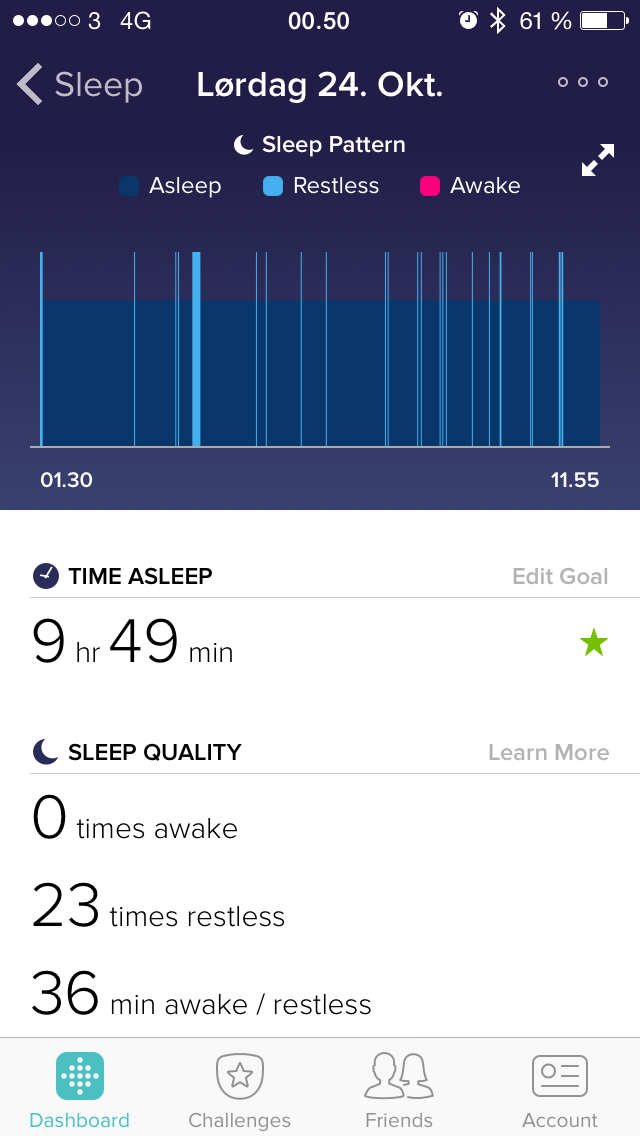
\includegraphics[width=\textwidth]{img/24-10-fitbit}
        \caption{Fitbit mobilephone application}
        \label{fig:fitbit0}
    \end{subfigure}
    ~ %add desired spacing between images, e. g. ~, \quad, \qquad, \hfill etc. 
      %(or a blank line to force the subfigure onto a new line)
    \begin{subfigure}[b]{0.45\textwidth}
        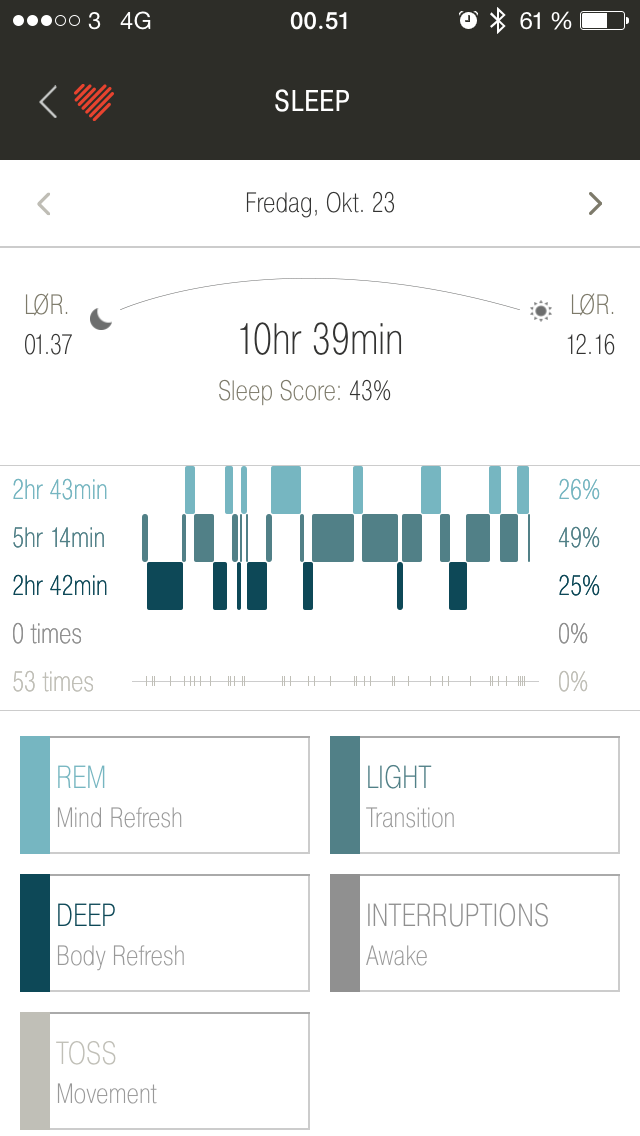
\includegraphics[width=\textwidth]{img/24-10-basis}
        \caption{BASIS mobilephone application}
        \label{fig:basis0}
    \end{subfigure}
    \caption{Fitbit vs. BASIS - an example sleep date night between 23-10-2015 and 24-10-2015. The self-reported sleep for this night was from 01:40 to 12:30. The evening before this sleep was spend going out.}
    \label{fig:pilot0}
\end{figure}

Figure \ref{fig:pilot1} shows the results of a more regular night, the night between a Sunday and Monday. Comparing the visualisations in both Figure \ref{fig:pilot0} and Figure \ref{fig:pilot1} it is clear that the two watches does not measure the exact same time for sleeping. The time of sleep between the days illustrated in Figure \ref{fig:pilot0} was from 01:40 to 12:30. It is also evident that the Basis Peak is measuring in more details than the Fitbit Surge. \\

Both watches have a second view in their application for the smartphones, a more detailed view. In Figure \ref{fig:pilot2} the second type of view is illustrated, and it is clear to see that Fitbit's view is far less detailed than the BASIS view. BASIS adds a timeline for sleep to visualise when REM, interruptions, and deep sleep occurred during the night. The difference between BASIS and Fitbit is illustrated in Figure \ref{fig:pilot1}.

\begin{figure}[H]
    \centering
    \begin{subfigure}[b]{0.45\textwidth}
        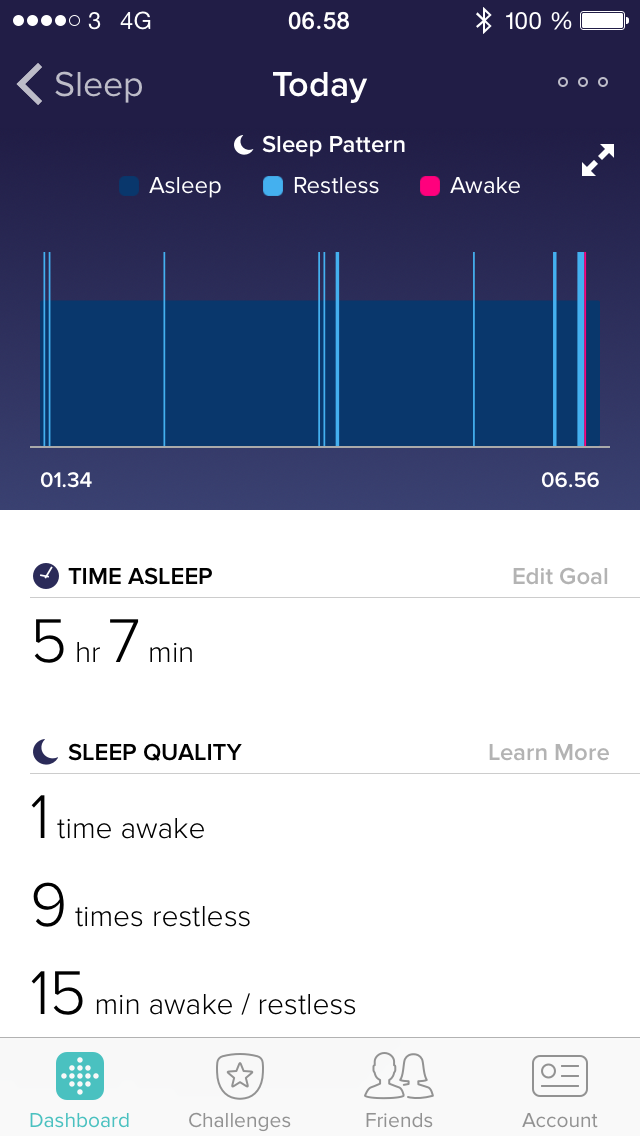
\includegraphics[width=\textwidth]{img/26-10-fitbit}
        \caption{Fitbit mobilephone application}
        \label{fig:fitbit1}
    \end{subfigure}
    ~ %add desired spacing between images, e. g. ~, \quad, \qquad, \hfill etc. 
      %(or a blank line to force the subfigure onto a new line)
    \begin{subfigure}[b]{0.45\textwidth}
        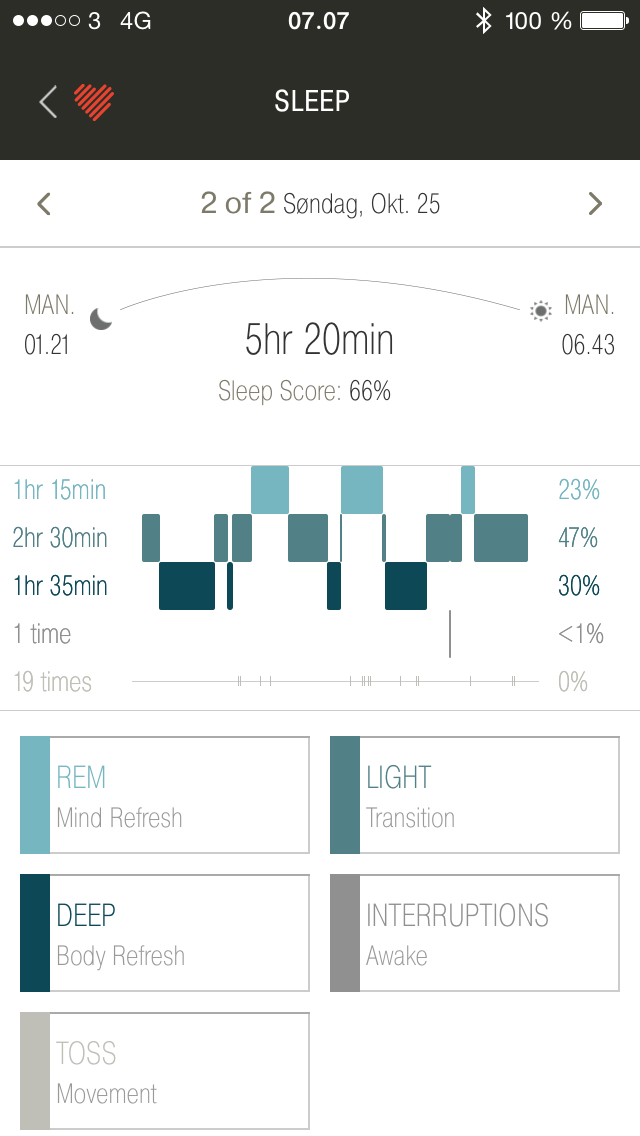
\includegraphics[width=\textwidth]{img/26-10-basis}
        \caption{BASIS mobilephone application}
        \label{fig:basis1}
    \end{subfigure}
    \caption{Fitbit vs. BASIS - night between 25-10-2015 and 26-10-2015, view 1. The self-reported sleep this night was from 01:20 to 6:30, and no alcohol was consumed before the sleep.}
    \label{fig:pilot1}
\end{figure}

\begin{figure}[H]
    \centering
    \begin{subfigure}[b]{0.45\textwidth}
        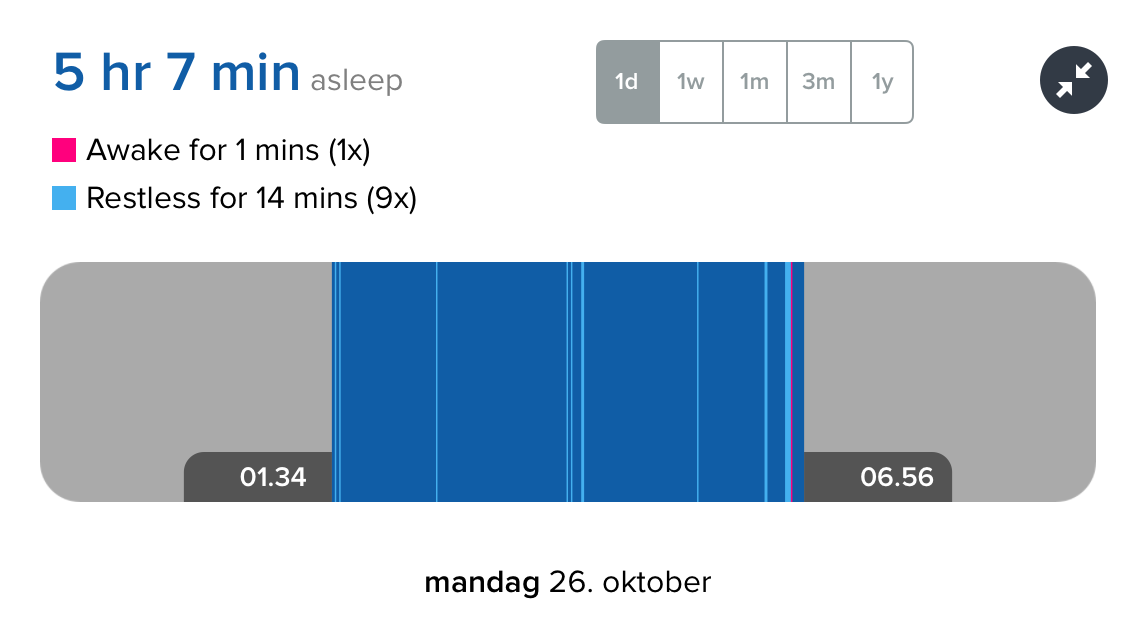
\includegraphics[width=\textwidth]{img/26-10-fitbit1}
        \caption{Fitbit mobilephone application}
        \label{fig:fitbit2}
    \end{subfigure}
    ~ %add desired spacing between images, e. g. ~, \quad, \qquad, \hfill etc. 
      %(or a blank line to force the subfigure onto a new line)
    \begin{subfigure}[b]{0.45\textwidth}
        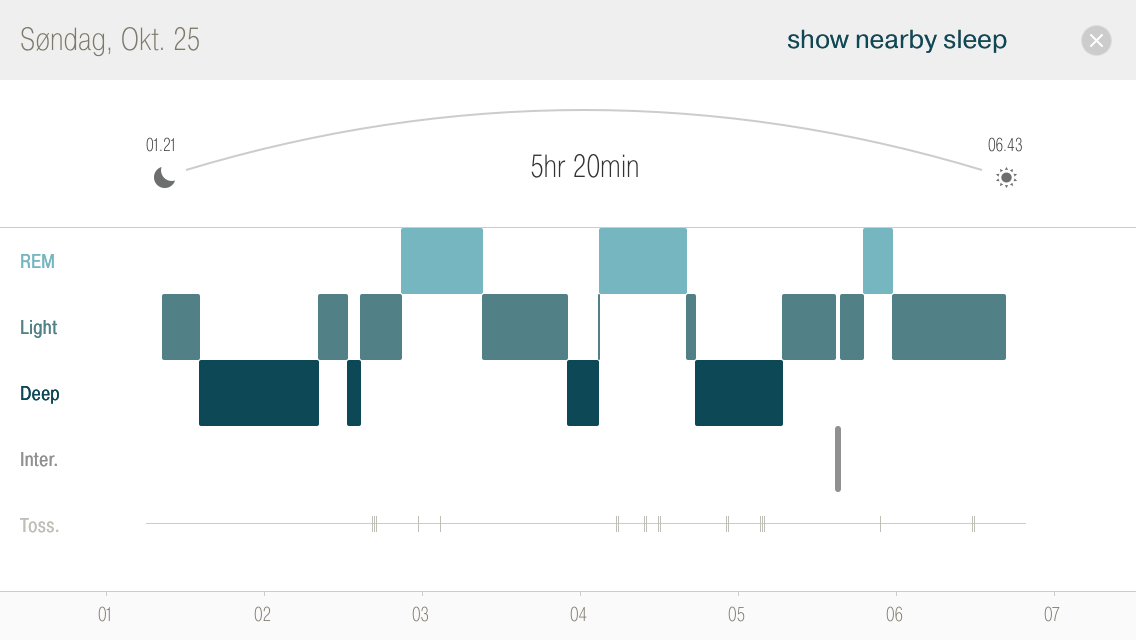
\includegraphics[width=\textwidth]{img/26-10-basis1}
        \caption{BASIS mobilephone application}
        \label{fig:basis2}
    \end{subfigure}
    \caption{Fitbit vs. BASIS - night between 25-10-2015 and 26-10-2015, view 2. The self-reported sleep this night was from 01:20 to 6:30, and no alcohol was consumed before the sleep.}
    \label{fig:pilot2}
\end{figure}

Extracting data from the BASIS watch was not possible through the user login at the website as first initiated, and the BASIS support team could not help either. Fortunately, there exists a third party script written in Python called Basis Retriever \cite{basis_retriever}. With that, it is possible to extract a CSV file from a given user that contains detailed information about the users sleep on a particular day. It is possible to download both for a single day, but also a summary for an entire month. Appendix \ref{sec:subset} contains a subset of how a CSV file with data from a single day is looking. \\

Because we could not extract the data collected in raw format from the Fitbit watch, and because the BASIS Peak watch was more precise in measuring sleep according to our examples in \ref{fig:pilot0} and Figure \ref{fig:pilot1}, it was decided that the BASIS watch was the best of the two, hence the one used in the study. \\

Several studies have validated heart rate as a way to measure sleep quality \cite{heartratesleep}\cite{heartrateagain}, and in 2015 Emil Jovanov \cite{EmilBasis} made a preliminary study on BASIS Peak with heart rate measurement as the focus. As his `ground truth' he used a Zephyr Bioharness 3 monitor and SOMNOscreen+ polysomnographic monitoring system from SOMNOmedics. For the watch, 11.2\% of records was missing, 1.43\% was missing from SOMNOscreen+, and the Zephyr Bioharness lost 1.74\% of records collected. The study analysed the difference between average heart rate measured by BASIS Peak and Zephyr Bioharness, which gave an average difference on 0.89 beats per minute (bpm) with standard deviation of 1.03 bpm, and a maximum difference of 3.13 bpm. \\

Jovanov concludes that the technology in smartwatches today is efficient enough to perform longitudinal monitoring and analysis on health and related trends. \\

The BASIS watch collects the following variables every minute: date and time, skin temperature, air temperature, heart rate, steps, galvanic skin response (gsr), calories, activity type (bike, manual, moderate activity, run, walk), sleep type (deep, REM, light, unknown), and toss and turns during sleep. 

\subsubsection{Day Reconstruction Method}
The Day Reconstruction Method (DRM) is a way to assess how the participants spend their time and how they experience it for the last 24 hours \cite{drm}. These DRM's was collected once a week from each participant over two periods of time, in the beginning of the data collection period (experiment \#1) and again in the beginning of the second data collection period (experiment \#2). We used the DRM's as validation points for specific days to check our theories and to validate the patterns derived from the data collected. \\

Next to this study, another thesis study was conducted with the title ``Factors Influencing Individual's Sleep Quality and Quantity'' \cite{kimie}. This study coded the answers from the participants into 15 different labels for categorising what influences sleep quality: silence (SIL), temperature (TEM), stressfree (STR), bedtime (BED), exercise (EXE), health (HEA), nonalcohol (NON), awake (AWA), breathing (BRE), music (MUS), darkness (DAR), meditate (MED), stimuli (STI), alone (ALO), and reading (REA). \\

The Danish Council on Health and Disease Prevention created a report in 2015 about sleep and health. That report supports some of Kimie Bodin Ryager's labels on factors influencing sleep quality and list the following lifestyle and psychological and behavioural advices on sleep: No coffee, alcohol, energy-rich and fatty foods before bedtime, be physical active during the day, optimal room temperature which for most individuals is 18-21 degrees Celcius, silence, no screen light from electronic devices, no light, go to bed and get up at regular times, no naps for more than 20 minutes, only use the bedroom for sleeping and sex, avoid negative thoughts \cite{vff}. 

\newpage 
\section{User Study and Setup}
\subsection{Timeline}
This project was initiated in September 2015 as a part-time master thesis, ending in February 2017. In October 2015 the recruitment process was started, and in November the first 9 participants started collecting data with four weekly DRM sessions. In December the 10th subject started and both in January and February 2016 a participant dropped out. In April another four weekly DRM sessions started, and in July the data collection ended and data analysis started. For a more detailed time plan, see Table \ref{tab:timeplan}. 

\begin{table}[H]
\center
\begin{footnotesize}
	\begin{tabular}{| c | c |}
	\hline
	\textbf{Month} & \textbf{Task} \\
	\hline
	September 2015 & Project initiated\\
	October 2015 & Literature study and recruitment process start\\
	November 2015 & Beginning of experiment \#1 \\
	 & Participant S11-15 and S17-20 starts collecting data \\
	December 2015 & Participant S16 starts collecting data\\
	January 2016 & Labelling first batch of DRM's \\
	February 2016 & \\
	March 2016 & End of experiment \#1 \\
	 & Preparing for next round of DRM's \\
	April 2016 & Beginning of experiment \#2 \\
	 & Participants fills out 4 new DRM's \\
	May 2016 & Labelling second batch of DRM's\\
	June 2016 & \\
	July 2016 & End of experiment \#2 \\
	 & Data collection ends and data analysis starts\\
	August 2016 & \\
	September 2016 & \\
	October 2016 & \\
	November 2016 & \\
	December 2016 & \\
	January 2017 & \\
	February 2017 & Thesis hand in on February 28$^{th}$\\
	\hline
	\end{tabular}
	\caption{Monthly based timeplan for project.}
	\label{tab:timeplan}
\end{footnotesize}
\end{table}

\subsection{Recruitment Process}
The target group for the study was students with Android OS smartphones with at least Android software version 4.4 to run the mQoL-log application, and Bluetooth version 2 or above to be able to connect to the BASIS peak application. The social network Facebook was used to get in contact with potential participants and hereafter most contact was happening via email. Before finalising the recruitment process we got the ethics protocol approved by the university ethics committee.

\subsection{Participants} \label{sec:participants}
The participants consists of 10 students primarily from University of Copenhagen (UCPH), and a single student from the IT University (ITU). They are all between the age of 18 and 30, and no one have children. In Table \ref{tab:partOv} an overview of the participant and their living conditions is shown. S11 lived with 2 friends before he moved in together with his girlfriend. S14 finished his master one month before the data collection period stopped and as seen in Figure \ref{fig:timeline} S19 dropped out of the experiment in January 2016 because the strap from the watch gave her a rash, and S18 dropped out in February because he lost his phone and bought an iPhone instead of an Android smartphone which made him unable to run the application from mQoL. In June S13 decided not to wear the watch any more due to the recommendations send out from BASIS regarding the heating issues. 

\begin{table}[H]
\center
\begin{footnotesize}
	\begin{tabular}{| c | c | c | c | c | c | c | c | c | c |}
	\hline
	\textbf{S\#} & \textbf{Gender} & \textbf{Age} & \textbf{University} & \textbf{Civil} & \textbf{Living-}\\
	 & \textbf{} & \textbf{} & \textbf{} & \textbf{status} & \textbf{conditions} \\
	
	\hline
	S11 & Male & 25-30 & UCPH & Relationship & With girlfriend from January 1, 2016 \\
	\hline
	S12 & Male & 18-24 & UCPH & Relationship & Apartment with friend\\
	\hline
	S13 & Male & 18-24 & UCPH & Single & Alone \\
	\hline
	S14 & Male & 25-30 & ITU & Relationship & Apartment with friend \\
	\hline
	S15 & Male & 18-24 & UCPH & Single & With parents  and 1 sibling\\
	\hline
	S16 & Male & 18-24 & UCPH & Single & Apartment with friend\\
	\hline
	S17 & Male & 18-24 & UCPH & Single & With parents and 2 siblings \\
	\hline
	S18 & Male & 18-24 & UCPH & Single & In a collective\\
	\hline
	S19 & Female & 18-24 & UCPH & Relationship & With parents and 1 sibling\\
	\hline
	S20 & Female & 18-24 & UCPH & Relationship & With boyfriend\\
	\hline
	\end{tabular}
	\caption{Participants overview. Only participants living with a boy/girlfriend shared bed/room with another person.}
	\label{tab:partOv}
\end{footnotesize}
\end{table}

Only two of the participants was master students, S11 and S14. S11 was writing on his dissertation thesis during the entire data collecting period (November to July) and S14 started his thesis work in February 2016 and finished it in mid June. In Table \ref{tab:part1v} it is shown what the participants studied at the time of the data collection, what level they were at, how many month left of the current level, how many hours they estimate they study every week, how many hours per week they work at a student job, and how many hours they exercise each week. For each participant we also received information about civil status (in a relationship or not), or if they lived alone, with roommate/girlfriend/boyfriend or parents. This information was retrieved by the initial survey.   

\begin{table}[H]
\center
\begin{footnotesize}
	\begin{tabular}{| c | c | c | c | c | c | c | c |}
	\hline
	\textbf{S\#} & \textbf{Study} & \textbf{Level} & \textbf{Months left} & \textbf{Study} & \textbf{Work} & \textbf{Exercise}\\
	 & & & & \textbf{hours/week} & \textbf{hours/week} & \textbf{hours/week}\\
	\hline
	S11 & Physics & Master & 18 & 36-40 & 6-10 & 6-10 \\
	\hline
	S12 & Computer Science & Bachelor & 10 & 36-40 & 6-10 & 0-5\\
	\hline
	S13 & Computer Science & Bachelor & 10 & 31-35 & 0 & 6-10\\
	\hline
	S14 & Games \& Technology & Master & 5 & 26-30 & 6-10 & 6-10\\
	\hline
	S15 & Computer Science & Bachelor & 34 & 36-40 & 0 & 0-5\\
	\hline
	S16 & Computer Science & Bachelor & 34 & 26-30 & 6-10 & 6-10\\
	\hline
	S17 & Computer Science & Bachelor & 20 & 16-20 & 0-5 & 6-10\\
	\hline
	S18 & Computer Science & Bachelor & 20 & 36-40 & 11-15 & 6-10\\
	\hline
	S19 & Computer Science & Bachelor & 12 & 36-40 & 0 & 0-5\\
	\hline
	S20 & Pharmacy & Bachelor & 21 & 31-35 & 0-5 & 0-5\\
	\hline
	\end{tabular}
	\caption{Participants workload overview in hours per week and line of study}
	\label{tab:part1v}
\end{footnotesize}
\end{table}

\subsection{Collected Data Summary}
In Figure \ref{fig:timeline} a timeline over the entire data collection period is illustrated showing when the participants started, dropped out and when exams periods and holidays was during this time. Participant numbers written in green symbols when the participant started collecting data, and the red is illustrating when the participant decided to drop out of the experiment. 

\begin{figure}[H]
    \centering
        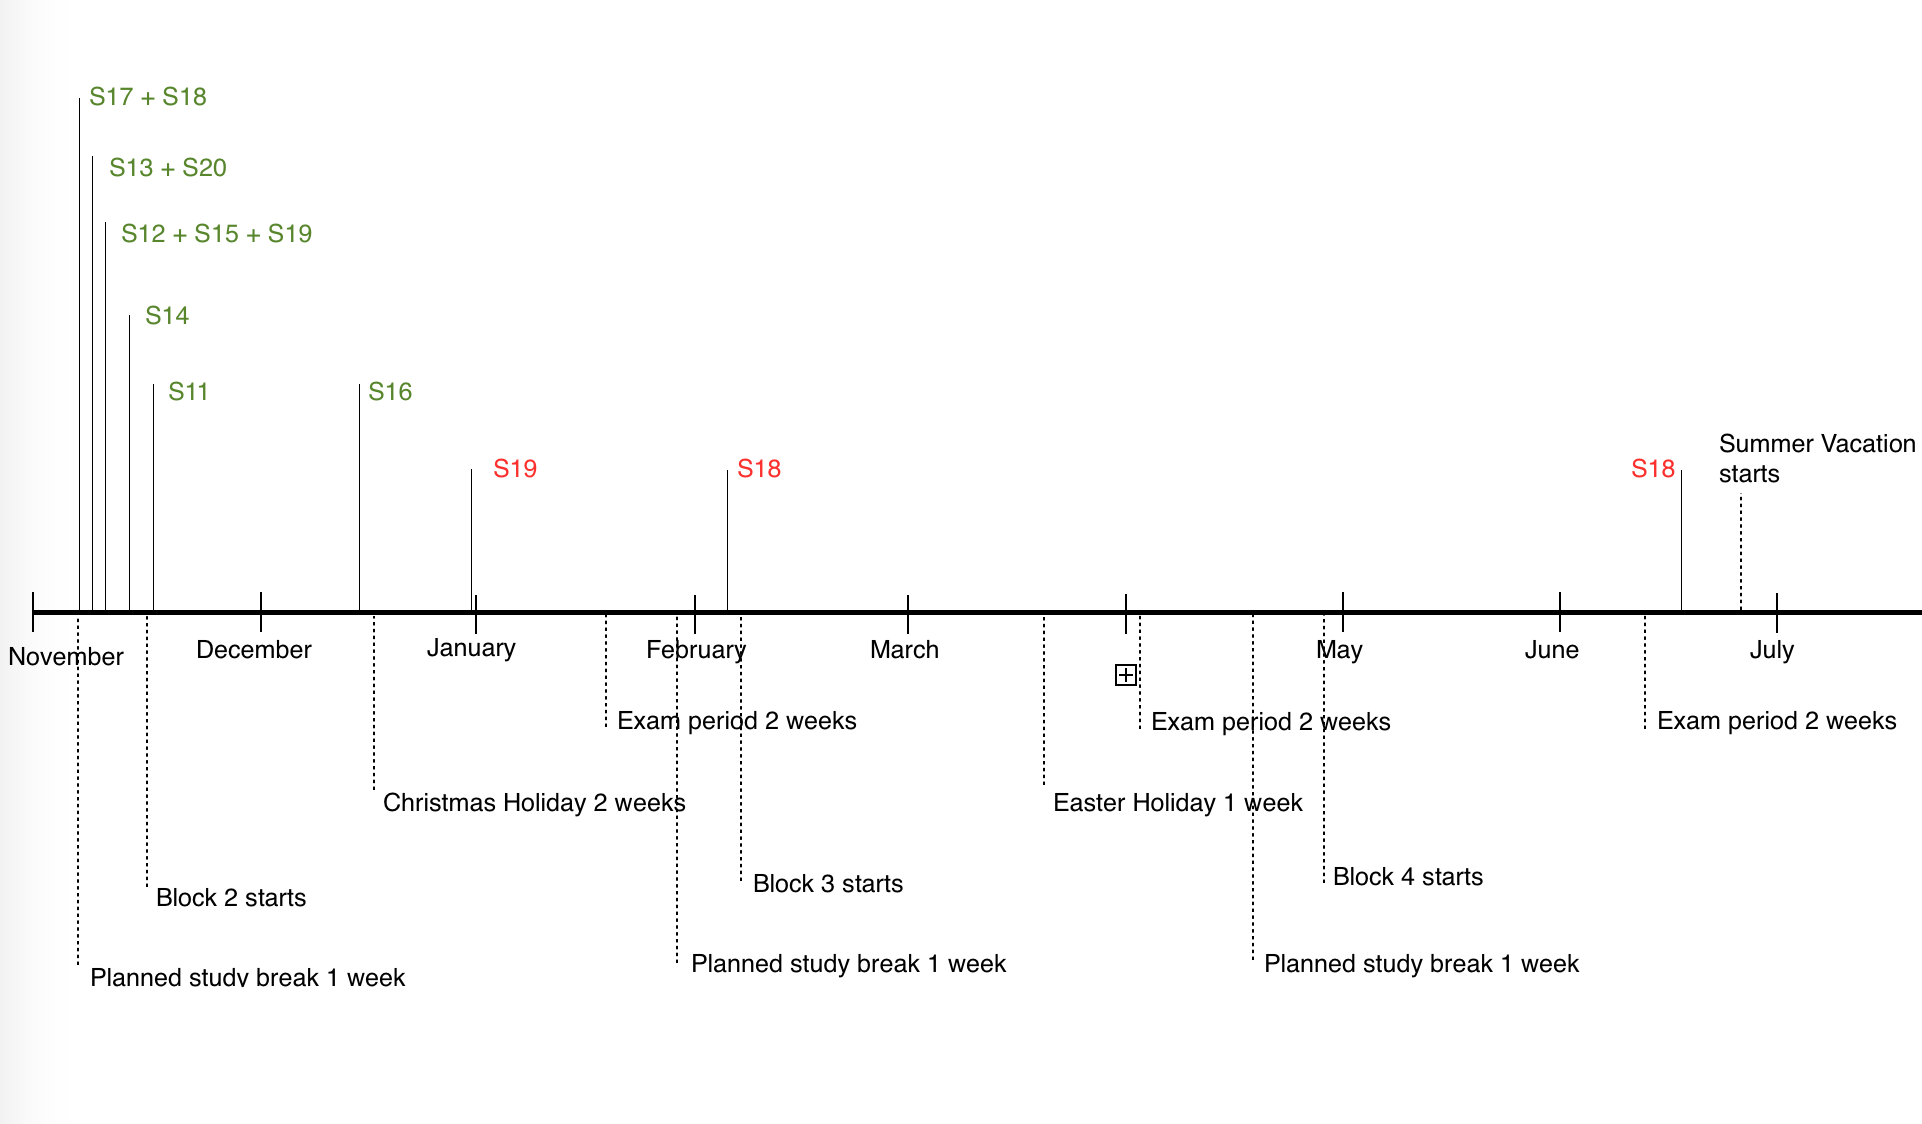
\includegraphics[width=\textwidth]{img/timeline}
        \caption{Timeline over entire data collection period}
        \label{fig:timeline}
\end{figure}

Besides the timeline in \ref{fig:timeline}, an illustration of the data collected with information on when DRM's was made, when exam periods, holidays, and significant days are shown in Figure \ref{fig:allAround}. Because the participants did not start the same day, November 20th, 2015 was chosen as the first day of the illustration, because at that day all nine participants starting in November have data. S16 started in December. Weekends are marked with blue, days with DRM's are marked with yellow, and December 18th, 2015 is marked with red, because eight out of ten participants entered the same yearly Christmas Dinner at Department of Computer Science, at University of Copenhagen. Symbols are marking Christmas Eve, New Years Eve, Ascension and Pentecost days, and a heart in two is illustrating when S20 broke up with her boyfriend. 

\begin{figure}[H]
    \centering
        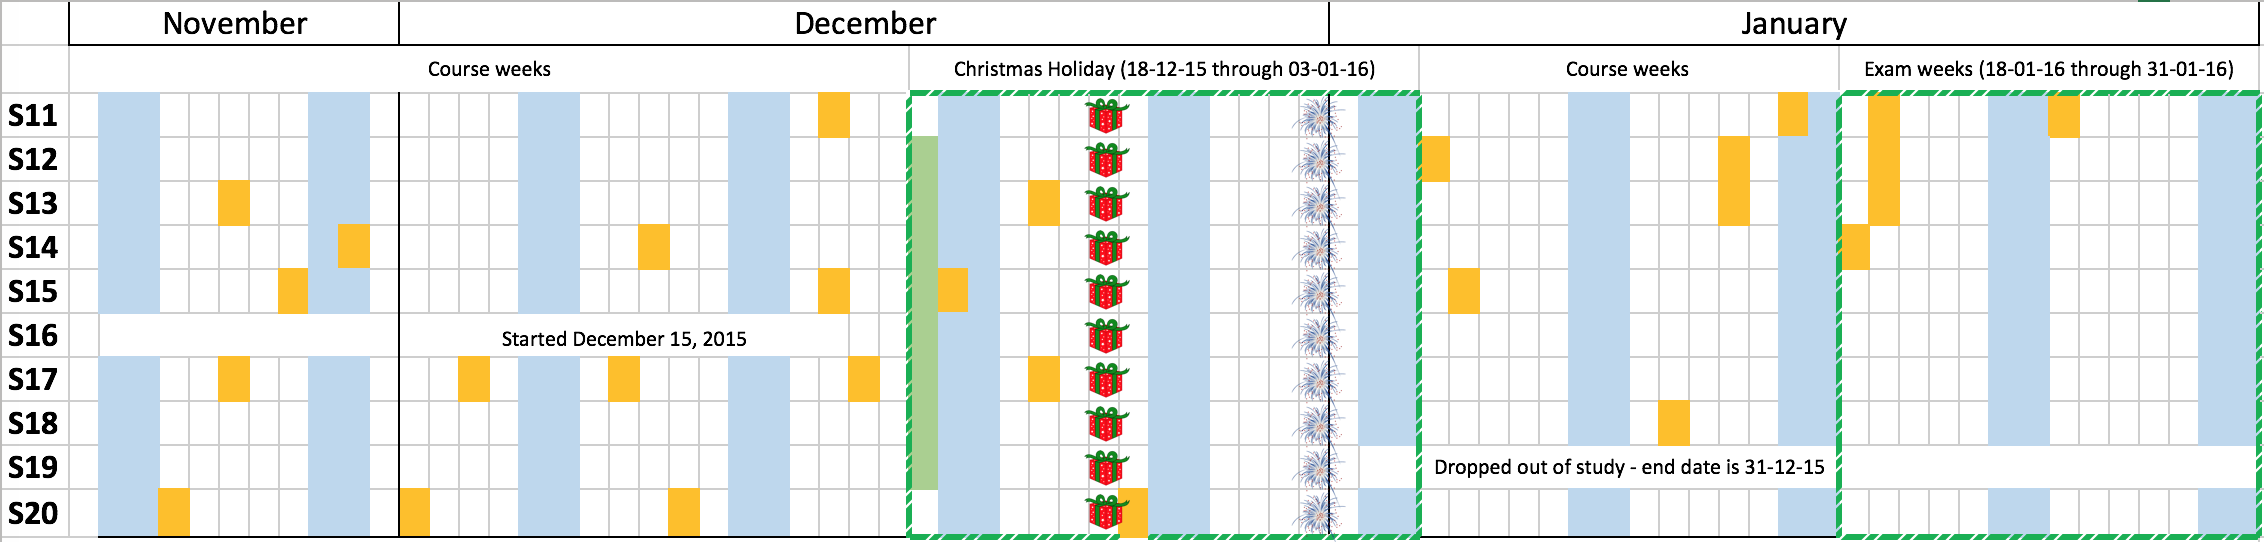
\includegraphics[width=\textwidth]{img/allAround1}
%        \caption{Illustration of data collecting from November 2015 through January 2016}
%        \label{fig:allAround1}
~
        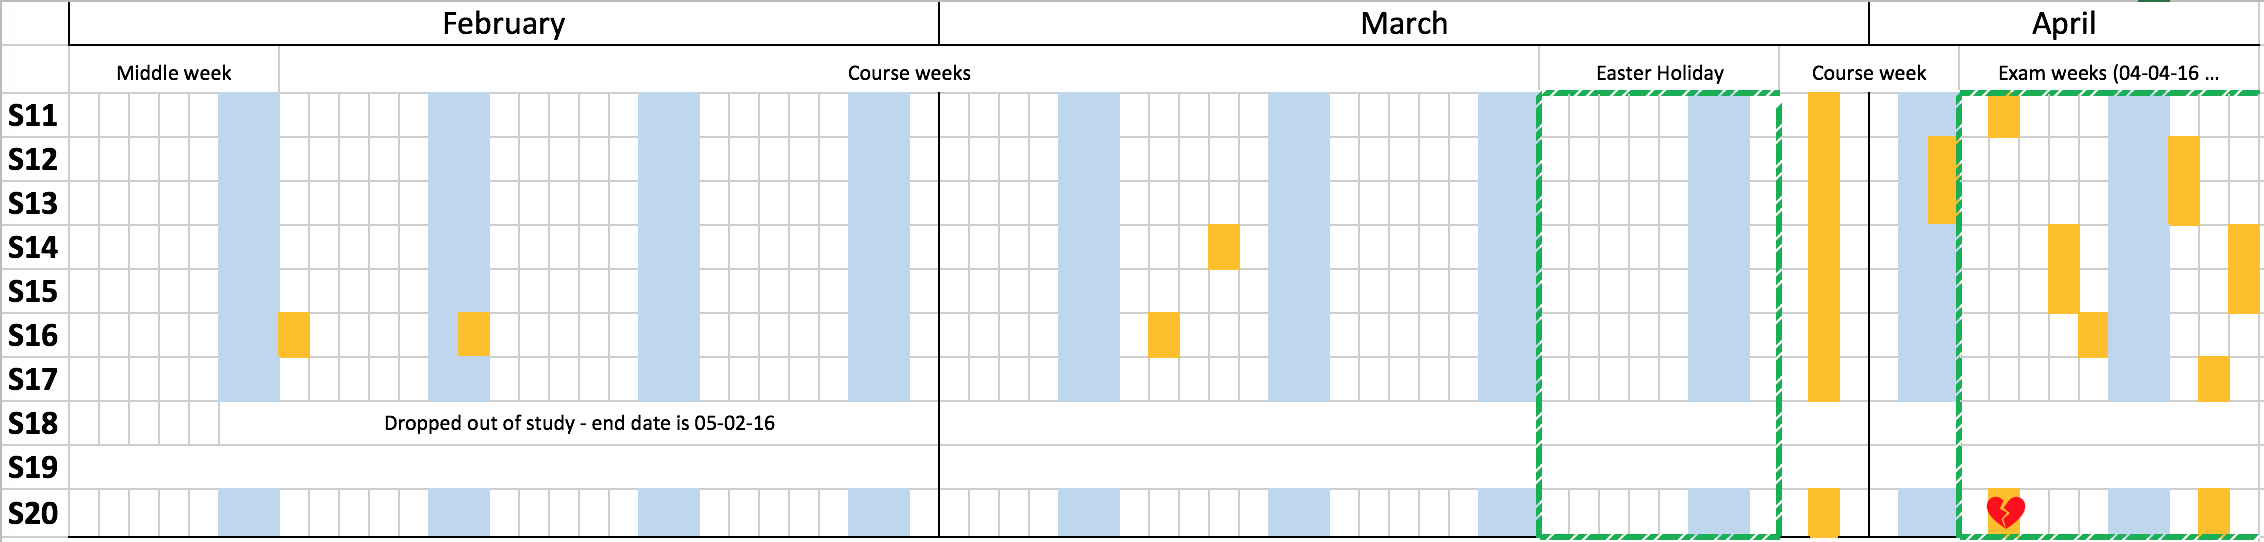
\includegraphics[width=\textwidth]{img/allAround2}
~
 		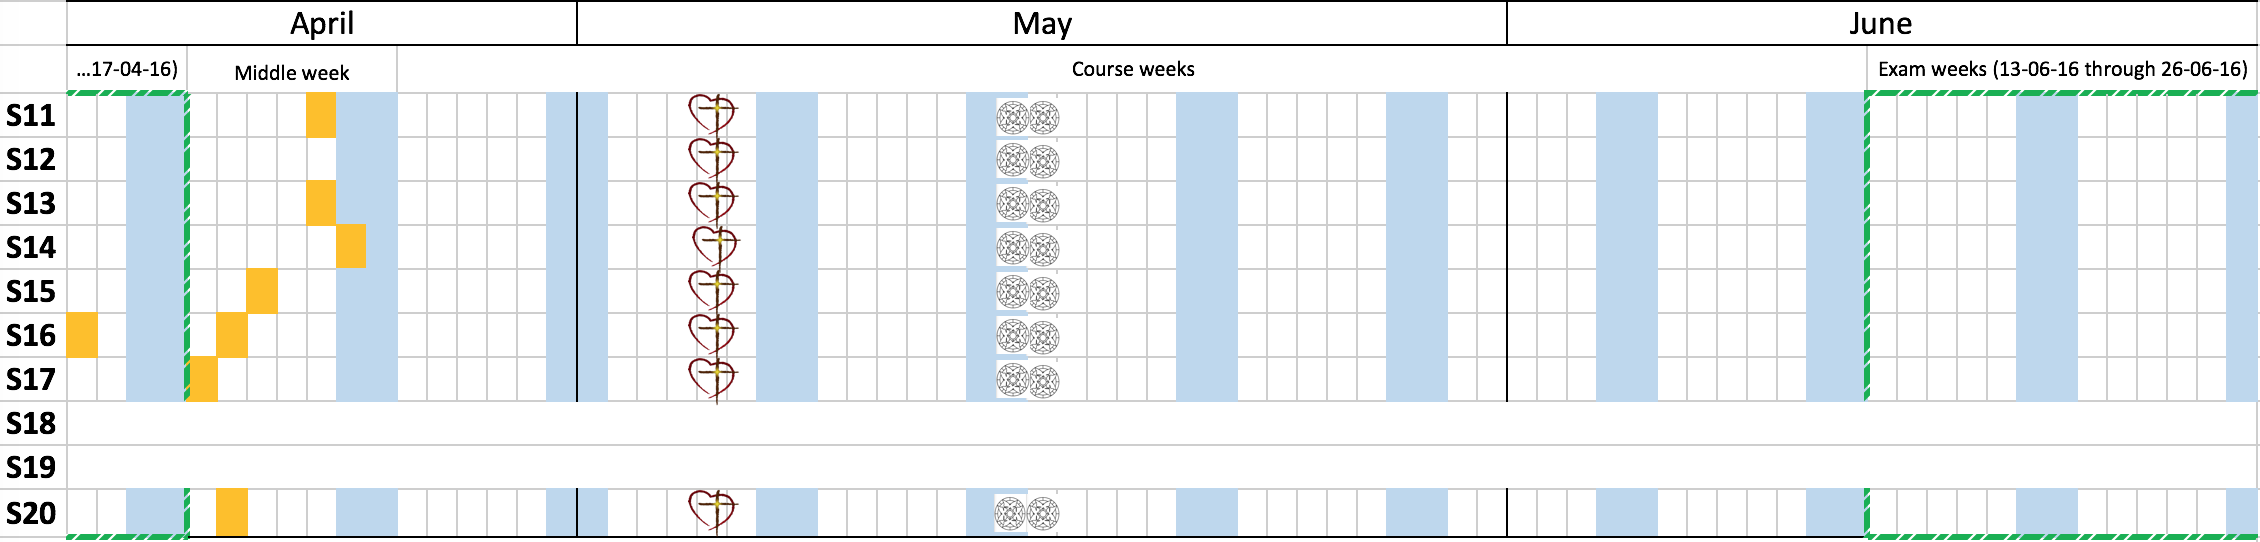
\includegraphics[width=\textwidth]{img/allAround3}
~
 		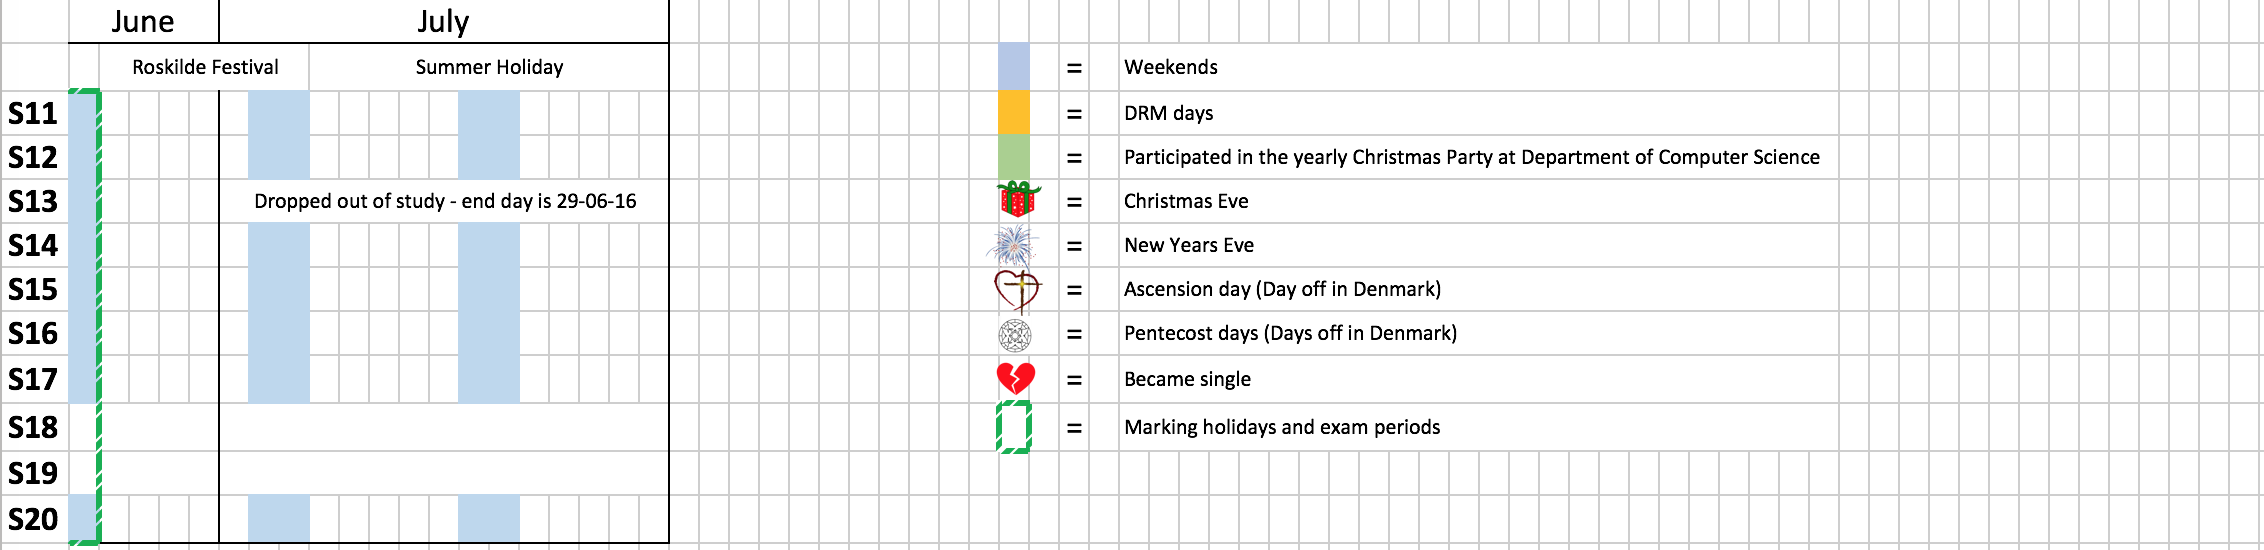
\includegraphics[width=\textwidth]{img/allAround4}       
       
        \caption{Illustration of data collecting from November 2015 through July 15, 2016}
        \label{fig:allAround}
\end{figure}

For later references and easier overview, Table \ref{tab:beginning} is showing exactly when each participant started collecting data, and when the participant stopped. In the rows for S13, S18, and S19 a reason is stated for why they stopped the data collecting before the official end day. 

\begin{table}[H]
\center
\begin{footnotesize}
	\begin{tabular}{| c | c | c | c | c |}
	\hline
	\textbf{S\#} & \textbf{Start date} & \textbf{Start time} & \textbf{End date} & \textbf{Reason} \\
	
	\hline
	S11 & 18-11-2015 & 05:38:00 PM & 15-07-2016 & -\\
	S12 & 11-11-2015 & 04:11:00 PM & 15-07-2016 & -\\
	S13 & 10-11-2015 & 11:54:00 AM & 29-06-2016 & Warnings from BASIS\\
	S14 & 15-11-2015 & 04:56:00 PM & 15-07-2016 & -\\
	S15 & 11-11-2015 & 02:32:00 PM & 15-07-2016 & -\\
	S16 & 15-12-2015 & 01:08:00 PM & 15-07-2016 & -\\
	S17 & 09-11-2015 & 03:59:00 PM & 15-07-2016 & -\\
	S18 & 09-11-2015 & 04:32:00 PM & 05-02-2016 & Changed to iPhone\\
	S19 & 11-11-2015 & 04:30:00 PM & 31-12-2015 & Allergic reaction from strap\\
	S20 & 10-11-2015 & 01:17:00 PM & 15-07-2016 & -\\
	\hline
	\end{tabular}
	\caption{Date overview of beginning and end for participants}
	\label{tab:beginning}
\end{footnotesize}
\end{table}
%%%%%%%%%%%%%%%%%%%%%%%%%%%%%%%%%%%%%%%%%%%%%%%%%%%%%%%%%%%%%%%
%%%%%%%%%%%%%%%%%%%%%%%%%%%%%%%%%%%%%%%%%%%%%%%%%%%%%%%%%%%%%%%
%%%%%%%%%%%%%%%%%%%%%%%%%%%%%%%%%%%%%%%%%%%%%%%%%%%%%%%%%%%%%%%
%%%%%%%%%%%%%%%%%%%%%%%%%%%%%%%%%%%%%%%%%%%%%%%%%%%%%%%%%%%%%%%
%%%%%%%%%%%%%%%%%%ABOVE IS SOMEWHAT PROOFREAD!%%%%%%%%%%%%%%%%%
%%%%%%%%%%%%%%%%%%%%%%%%%%%%%%%%%%%%%%%%%%%%%%%%%%%%%%%%%%%%%%%
%%%%%%%%%%%%%%%%%%%%%%%%%%%%%%%%%%%%%%%%%%%%%%%%%%%%%%%%%%%%%%%
%%%%%%%%%%%%%%%%%%%%%%%%%%%%%%%%%%%%%%%%%%%%%%%%%%%%%%%%%%%%%%%
%%%%%%%%%%%%%%%%%%%%%%%%%%%%%%%%%%%%%%%%%%%%%%%%%%%%%%%%%%%%%%%
%%%%%%%%%%%%%%%%%%%%%%%%%%%%%%%%%%%%%%%%%%%%%%%%%%%%%%%%%%%%%%%

\newpage
\section{Data Collection}
This chapter is about the data collection. Data was collected from November 2015 to mid July 2016, and split into two sessions; experiment 1 and experiment 2. The first experiment run from when the participant starts through March 2016, and the second run from April 1, 2016 to July 15, 2016 when the data collection ended. \\

The data from experiment 1 was used as learning data, and the data from experiment 2 was used to check our results from experiment 1. 

\subsection{Experiment \#1}
Not researching on the quality of the data but only the quantity, the amount of minutes from when a participant started until March 31 was calculated. Table \ref{tab:totalMinutesWatch} is showing how many minutes with any kind of data the Basis Retriever could export to the daily .CSV files from the watches. Table \ref{tab:totalMinutesWatch} is not differencing between what kind of data the columns contains, only if there is data in them. Later on the results from the quality is illustrated. 

\begin{table}[H]
\center
\begin{footnotesize}
	\begin{tabular}{| c | c || c | c | c | c | c | c | c | c | c |}
	\hline
	\textbf{S\#} & \textbf{Total} & \textbf{Skin} & \textbf{Air} & \textbf{Heart} & \textbf{Steps} & \textbf{GSR} & \textbf{Calories} & \textbf{Activity} & \textbf{Sleep} & \textbf{Toss}\\
	 & & \textbf{temp} & \textbf{temp} & \textbf{rate} & & & & \textbf{type} & \textbf{type} & \textbf{turn}\\
	
	\hline
	S11 & 193341 & 182211 & 182241 & 184092 & 148602 & 180318 & 151420 & 10502 & 58034 & 5464\\
	\hline
	S12 & 203508 & 173042 & 173042 & 173757 & 191506 & 172187 & 191506 & 5059 & 58040 & 4351 \\
	\hline
	S13 & 205205 & 171705 & 171705 & 173295 & 205008 & 169483 & 205008 & 6552 & 51334 & 3070\\
	\hline
	S14 & 197703 & 181936 & 181139 & 182364 & 197511 & 181675 & 197511 & 9553 & 61673 & 2899 \\
	\hline
	S15 & 203607 & 180089 & 180139 & 181608 & 200969 & 179137 & 200969 & 6184 & 65580 & 6364 \\
	\hline
	S16 & 154731 & 73809 & 73809 & 75414 &136676 & 65852 & 136406 & 2978 & 33879 & 2386\\
	\hline
	S17 & 206402 & 171272 & 171272 & 175968 & 204397 & 162084 & 204397 & 15106 & 50219 & 5033\\
	\hline
	S18 & 127167 & 108515 &108515 & 108672 & 126539 & 108449 & 126539 & 8059 & 37288 & 3702 \\
	\hline
	S19 & 72449 & 49720 & 49720 & 49916 & 72401 & 49451 & 72401 & 2308 & 16745 & 1381 \\
	\hline
	S20 & 205122 & 187751 & 187751 & 190439 & 204821 & 183793 & 204811 & 6280 & 62119 & 4994\\
	\hline
	\end{tabular}
	\caption{Minutes with any kind of data from beginning to March 31, 2016 - smartwatch.}
	\label{tab:totalMinutesWatch}
\end{footnotesize}
\end{table}

In table \ref{tab:daysNightsExp1} a total number of days and nights with any kind of data is listed. The definition of days and nights is defined like this: \todo{FIND SOMETHING TO WRITE HERE}. ALSO WRITE SOMETHING ABOUT HOW YOU DEFINED WHEN A DAY/NIGHT IS VALID OR INVALID AND WHY!

\begin{table}[H]
\center
\begin{footnotesize}
	\begin{tabular}{| c | c | c || c | c | c | c | c | c | c | c |}
	\hline
	\textbf{S\#} & \textbf{Total} & \textbf{Total} & \textbf{Days} & \textbf{Nights} \\
	& \textbf{Days} & \textbf{Nights} & & \\
	\hline
	S11 & & & & \\
	S12 & & & & \\
	S13 & & & & \\
	S14 & & & & \\
	S15 & & & & \\
	S16 & & & & \\
	S17 & & & & \\
	S18 & & & & \\
	S19 & & & & \\
	S20 & & & & \\
	\hline
	\end{tabular}
	\caption{Days and nights with any kind of data from beginning to March 31, 2016 - smartwatch.}
	\label{tab:daysNightsExp1}
\end{footnotesize}
\end{table}

In Table \ref{tab:averageTotal}, a total average of the first six columns of the BASIS retriever data is shown. For skin- and air temperature, heart rate, and GSR, the average value is calculated based on each data entry in the data set (i.e. seconds) whereas the average for steps and calories is calculated based on a total for each day. 

\begin{table}[H]
\center
\begin{footnotesize}
	\begin{tabular}{| c | c | c | c | c | c | c | c | c | c |}
	\hline
	\textbf{S\#} & \textbf{Skin} & \textbf{Air} & \textbf{Heart} & \textbf{Steps} & \textbf{GSR} & \textbf{Calories}\\
	 & \textbf{temp} & \textbf{temp} & \textbf{rate} & & & \\
	
	\hline
	S11 & 30.97 & 29.22 & 77.42 & 6981 & 0.125 & 2545 \\
	\hline
	S12 & 31.29 & 29.13 & 73.04 & 3594 & 0.051 & 1969 \\
	\hline
	S13 & 30.76 & 28.65 & 73.93 & 4037 & 0.088 & 2771 \\
	\hline
	S14 & 30.65 & 28.78 & 77.55 & 4124 & 0.591 & 4679 \\
	\hline
	S15 & 31.46 & 29.89 & 75.34 & 4914 & 0.013 & 2426 \\
	\hline
	S16 & 30,00 & 28.56 & 73.15 & 2948 & 0.031 & 4148 \\
	\hline
	S17 & 30.95 & 29.34 & 77.55 & 8302 & 0.067 & 2621 \\
	\hline
	S18 & 30.06 & 28.26 & 82.18 & 6860 & 0.592 & 3490 \\
	\hline
	S19 & 32.99 & 31.62 & 85.65 & 4314 & 0.308 & 1943 \\
	\hline
	S20 & 30.92 & 29.06 & 75.27 & 5159 & 0.001 & 2063 \\
	\hline
	\end{tabular}
	\caption{Average in total from beginning to March 31, 2016 - smartwatch, column 1-6.}
	\label{tab:averageTotal}
\end{footnotesize}
\end{table}

\newpage
\begin{table}[H]
\center
\begin{footnotesize}
	\begin{tabular}{| c | c | c | c | c | c | c | c | c | c |}
	\hline
	\textbf{S\#} & \textbf{November} & \textbf{December} & \textbf{January} & \textbf{February} & \textbf{March} \\
	
	\hline
	S11 & 30.60 & 31.27 & 30.92 & 30.86 & 31.20\\
	\hline
	S12 & 31.39 & 31.37 & 31.09 & 31.15 & 31.44\\
	\hline
	S13 & 31.08 & 31.23 & 30.64 & 30.38 & 30.48\\
	\hline
	S14 & 30.53 & 30.60 & 31.01 & 30.75 & 30.37\\
	\hline
	S15 & 31.64 & 31.71 & 31.40 & 31.20 & 31.38\\
	\hline
	S16 & - & 30.25 & 29.67 & 30.06 & 30.02\\
	\hline
	S17 & 31.29 & 30.95 & 30.88 & 30.73 & 30.88\\
	\hline
	S18 & 30.03 & 29.23 & 30.00 & 30.72 & - \\
	\hline
	S19 & 32.87 & 33.12 & - & - & -\\
	\hline
	S20 & 30.81 & 31.12 & 30.83 & 30.79 & 31.03\\
	\hline
	\end{tabular}
	\caption{Average skin temperature per month from beginning to March 31, 2016 - smartwatch.}
	\label{tab:skinMinutesWatch}
\end{footnotesize}
\end{table}

\begin{figure}[H]
    \centering
    \begin{subfigure}[b]{0.30\textwidth}
        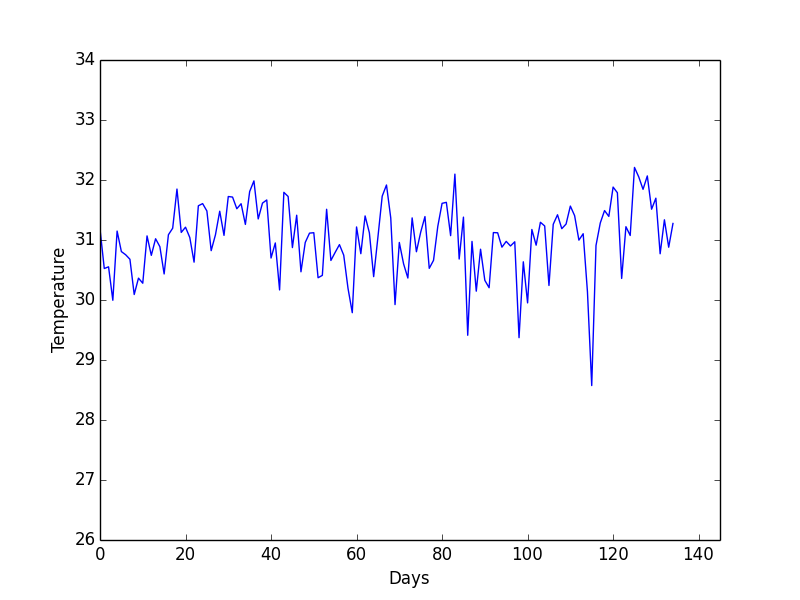
\includegraphics[width=\textwidth]{img/graphs/11-skintemp-1}
        \caption{S11}
        \label{fig:s11ST}
    \end{subfigure}
    ~ %add desired spacing between images, e. g. ~, \quad, \qquad, \hfill etc. 
      %(or a blank line to force the subfigure onto a new line)
    \begin{subfigure}[b]{0.30\textwidth}
        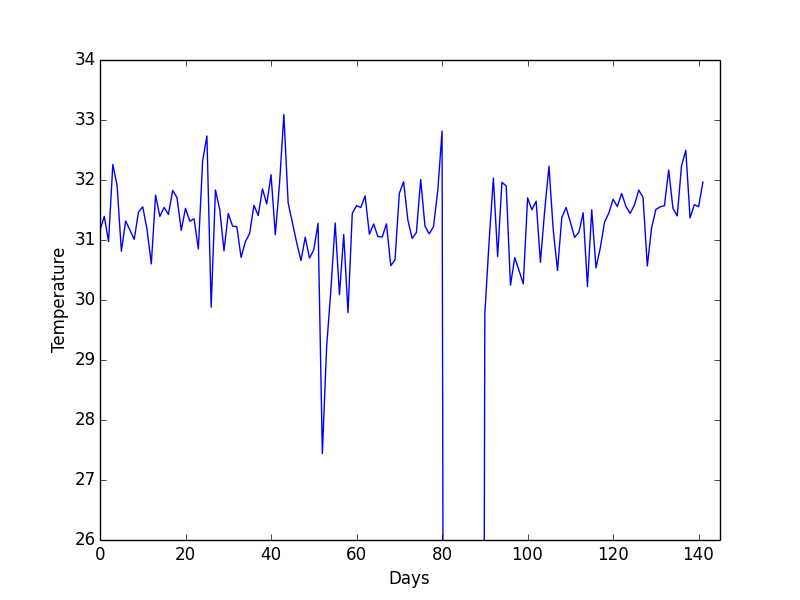
\includegraphics[width=\textwidth]{img/graphs/12-skintemp-1}
        \caption{S12}
        \label{fig:s12ST}
    \end{subfigure}
    ~ %add desired spacing between images, e. g. ~, \quad, \qquad, \hfill etc. 
      %(or a blank line to force the subfigure onto a new line)
    \begin{subfigure}[b]{0.30\textwidth}
        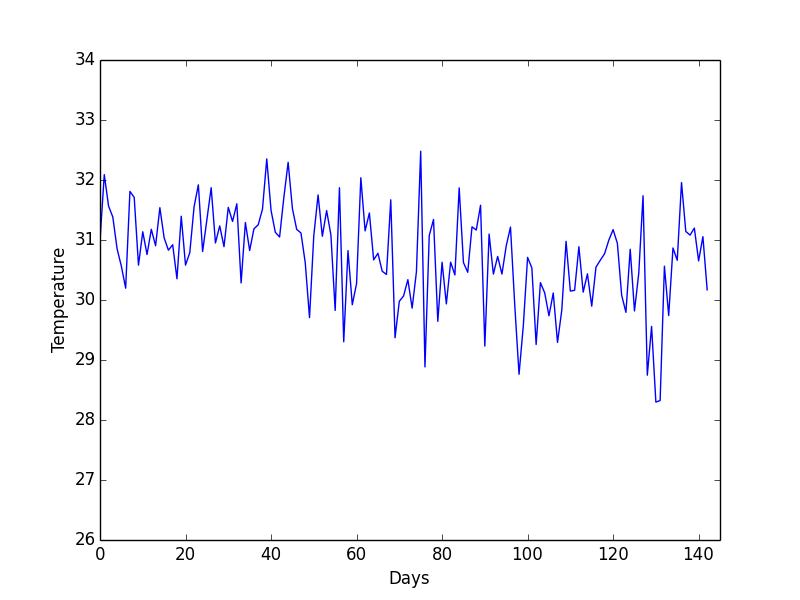
\includegraphics[width=\textwidth]{img/graphs/13-skintemp-1}
        \caption{S13}
        \label{fig:s13ST}
    \end{subfigure}
    ~ %add desired spacing between images, e. g. ~, \quad, \qquad, \hfill etc. 
      %(or a blank line to force the subfigure onto a new line)
    \begin{subfigure}[b]{0.30\textwidth}
        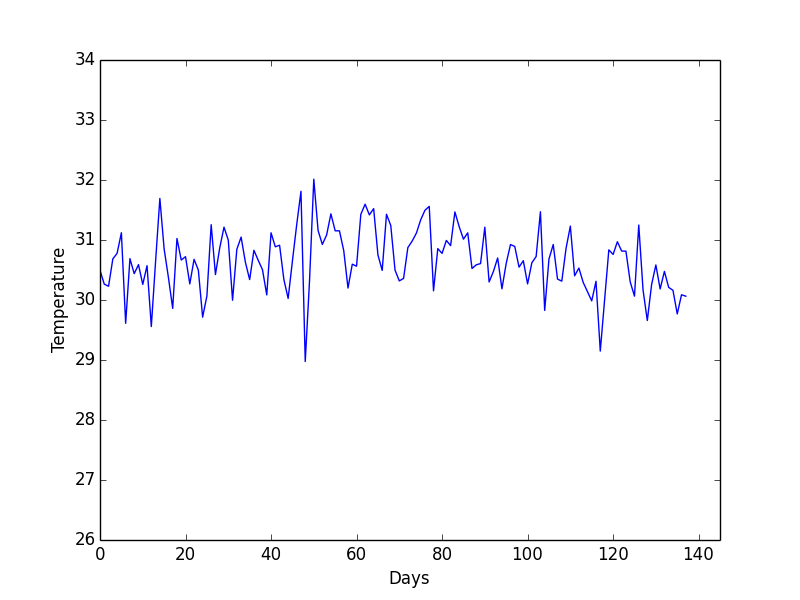
\includegraphics[width=\textwidth]{img/graphs/14-skintemp-1}
        \caption{S14}
        \label{fig:s14ST}
    \end{subfigure}
    ~ %add desired spacing between images, e. g. ~, \quad, \qquad, \hfill etc. 
      %(or a blank line to force the subfigure onto a new line)
    \begin{subfigure}[b]{0.30\textwidth}
        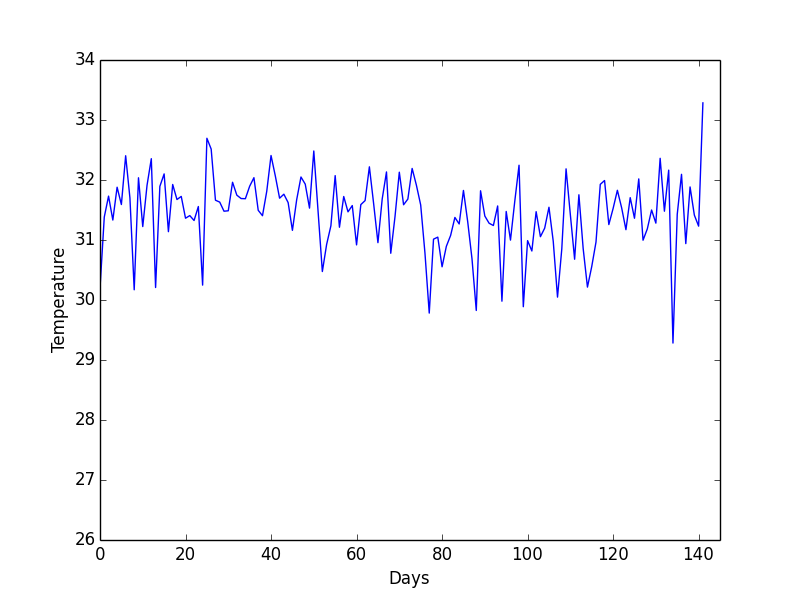
\includegraphics[width=\textwidth]{img/graphs/15-skintemp-1}
        \caption{S15}
        \label{fig:s15ST}
    \end{subfigure}
    ~ %add desired spacing between images, e. g. ~, \quad, \qquad, \hfill etc. 
      %(or a blank line to force the subfigure onto a new line)
    \begin{subfigure}[b]{0.30\textwidth}
        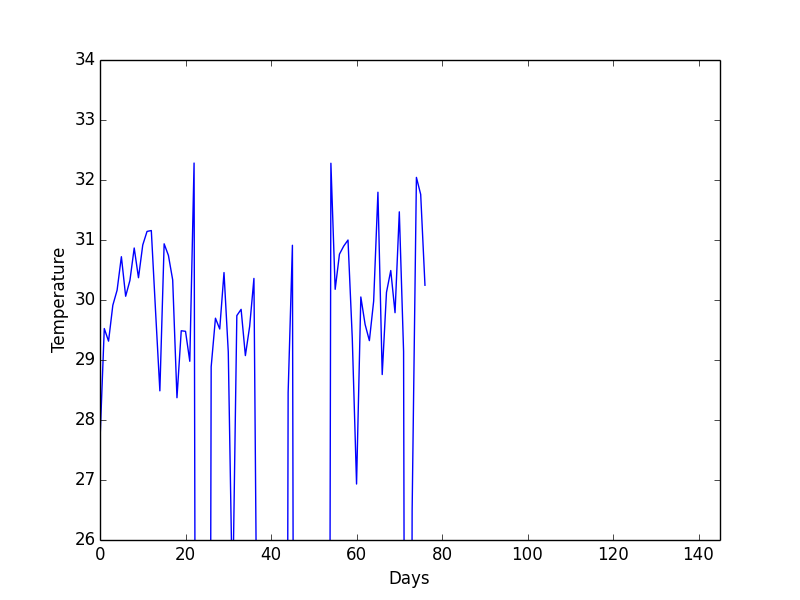
\includegraphics[width=\textwidth]{img/graphs/16-skintemp-1}
        \caption{S16}
        \label{fig:s16ST}
    \end{subfigure}
    ~ %add desired spacing between images, e. g. ~, \quad, \qquad, \hfill etc. 
      %(or a blank line to force the subfigure onto a new line)
    \begin{subfigure}[b]{0.2\textwidth}
        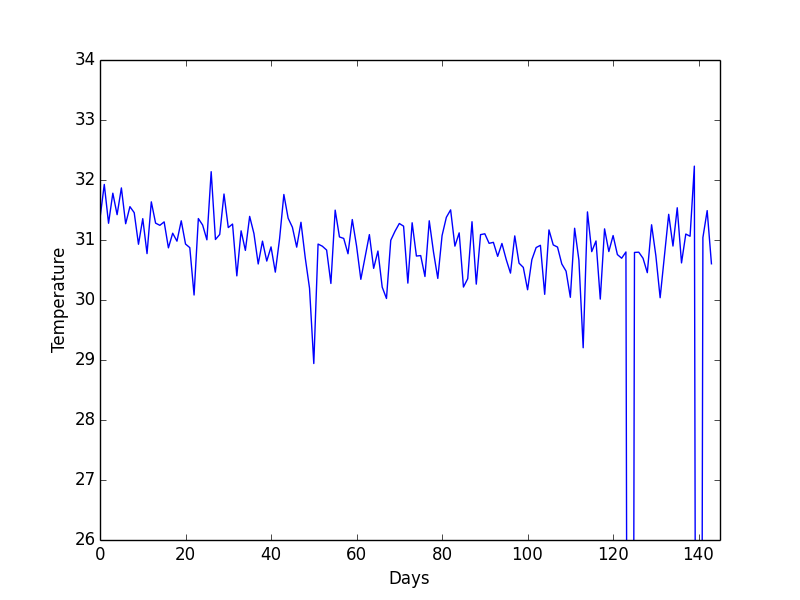
\includegraphics[width=\textwidth]{img/graphs/17-skintemp-1}
        \caption{S17}
        \label{fig:s17ST}
    \end{subfigure}
    ~ %add desired spacing between images, e. g. ~, \quad, \qquad, \hfill etc. 
      %(or a blank line to force the subfigure onto a new line)
    \begin{subfigure}[b]{0.2\textwidth}
        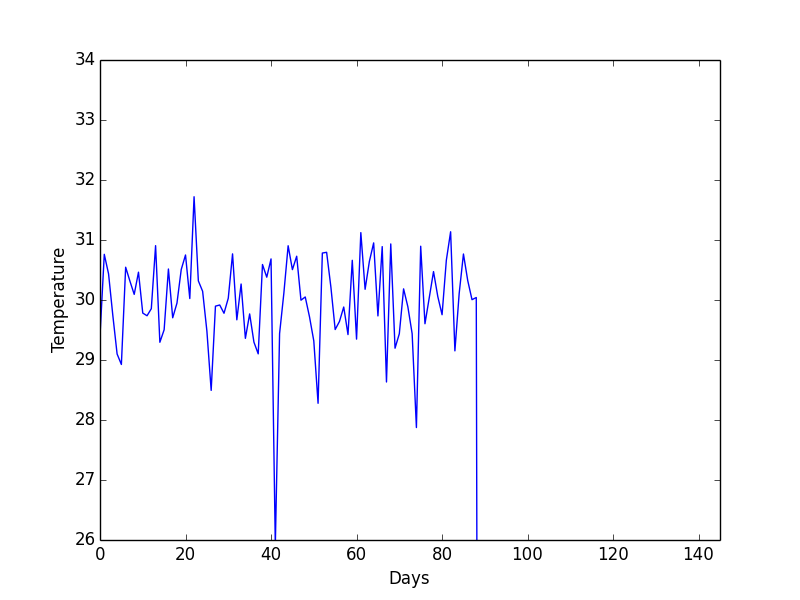
\includegraphics[width=\textwidth]{img/graphs/18-skintemp-1}
        \caption{S18}
        \label{fig:s18ST}
    \end{subfigure}
    ~ %add desired spacing between images, e. g. ~, \quad, \qquad, \hfill etc. 
      %(or a blank line to force the subfigure onto a new line)
    \begin{subfigure}[b]{0.2\textwidth}
        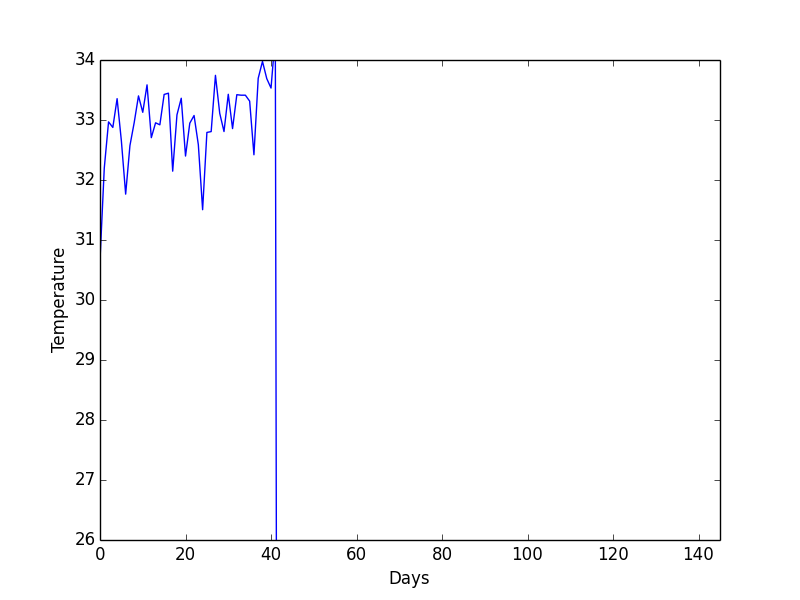
\includegraphics[width=\textwidth]{img/graphs/19-skintemp-1}
        \caption{S19}
        \label{fig:s19ST}
    \end{subfigure}
    ~ %add desired spacing between images, e. g. ~, \quad, \qquad, \hfill etc. 
      %(or a blank line to force the subfigure onto a new line)
    \begin{subfigure}[b]{0.2\textwidth}
        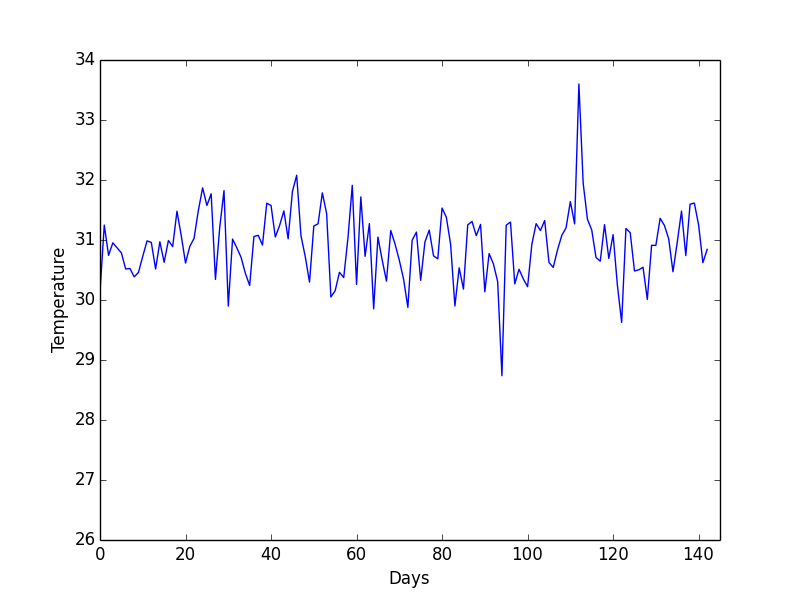
\includegraphics[width=\textwidth]{img/graphs/20-skintemp-1}
        \caption{S20}
        \label{fig:s20ST}
    \end{subfigure}
    \caption{Average skin temperature on daily basis from beginning through March}
    \label{fig:avgSkinTemp1}
\end{figure}


\begin{table}[H]
\center
\begin{footnotesize}
	\begin{tabular}{| c | c | c | c | c | c | c | c | c | c |}
	\hline
	\textbf{S\#} & \textbf{November} & \textbf{December} & \textbf{January} & \textbf{February} & \textbf{March} \\
	
	\hline
	S11 & 28.71 & 29.41 & 29.20 & 29.11 & 29.66\\
	\hline
	S12 & 29.18 & 29.25 & 29.00 & 28.99 & 29.24	\\
	\hline
	S13 & 28.96 & 29.17 & 28.57 & 28.19 & 28.36\\
	\hline
	S14 & 28.60 & 28.64 & 29.22 & 28.95 & 28.50\\
	\hline
	S15 & 30.08 & 30.21 & 29.85 & 29.59 & 29.73\\
	\hline
	S16 & - & 28.82 & 28.26 & 28.65 & 28.61\\
	\hline
	S17 & 29.78 & 29.35 & 29.25 & 29.14 & 29.18\\
	\hline
	S18 & 28.30 & 28.21 & 28.11 & 28.43 & - \\
	\hline
	S19 & 31.48 & 31.76 & - & - & -\\
	\hline
	S20 & 28.83 & 29.25 & 28.90 & 28.99 & 29.34\\
	\hline
	\end{tabular}
	\caption{Average air temperature per month from beginning through March, 2016 - smartwatch.}
	\label{tab:airMinutesWatch}
\end{footnotesize}
\end{table}

\begin{figure}[H]
    \centering
    \begin{subfigure}[b]{0.30\textwidth}
        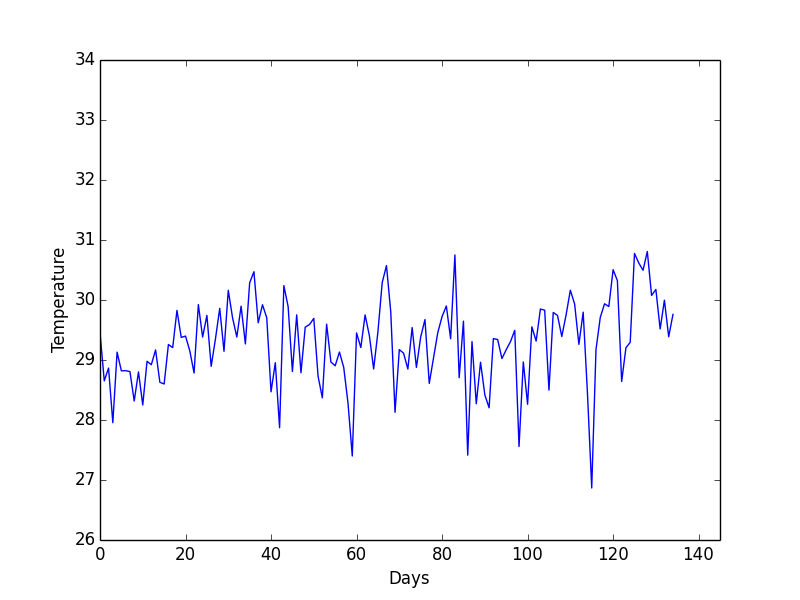
\includegraphics[width=\textwidth]{img/graphs/11-airtemp-1}
        \caption{S11}
        \label{fig:s11AT}
    \end{subfigure}
    ~ %add desired spacing between images, e. g. ~, \quad, \qquad, \hfill etc. 
      %(or a blank line to force the subfigure onto a new line)
    \begin{subfigure}[b]{0.30\textwidth}
        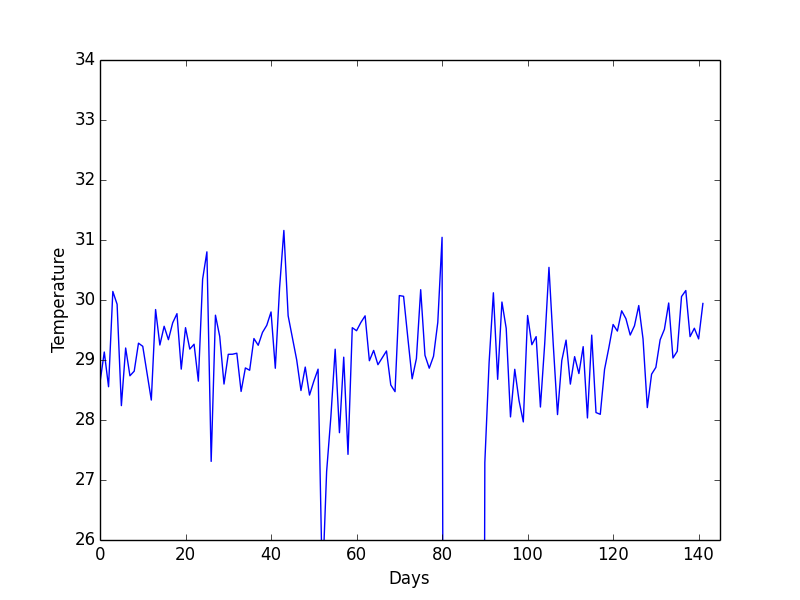
\includegraphics[width=\textwidth]{img/graphs/12-airtemp-1}
        \caption{S12}
        \label{fig:s12AT}
    \end{subfigure}
    ~ %add desired spacing between images, e. g. ~, \quad, \qquad, \hfill etc. 
      %(or a blank line to force the subfigure onto a new line)
    \begin{subfigure}[b]{0.30\textwidth}
        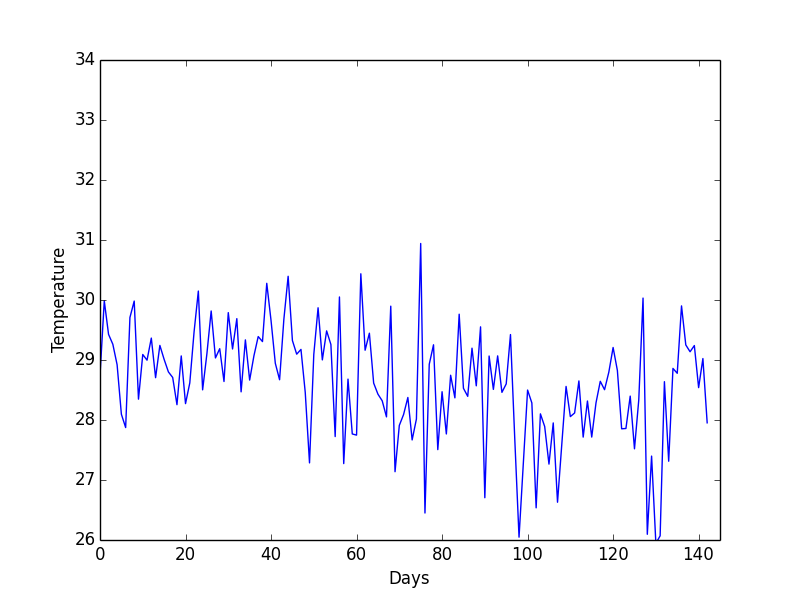
\includegraphics[width=\textwidth]{img/graphs/13-airtemp-1}
        \caption{S13}
        \label{fig:s13AT}
    \end{subfigure}
    ~ %add desired spacing between images, e. g. ~, \quad, \qquad, \hfill etc. 
      %(or a blank line to force the subfigure onto a new line)
    \begin{subfigure}[b]{0.30\textwidth}
        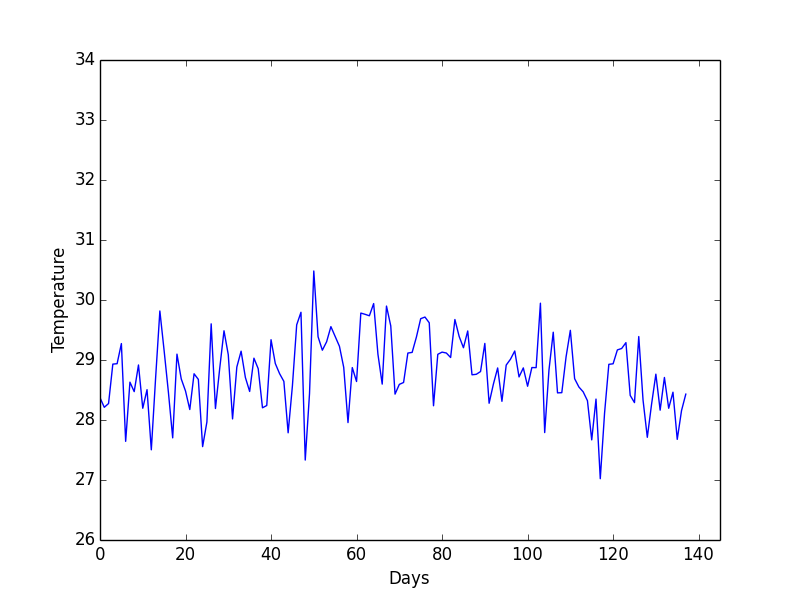
\includegraphics[width=\textwidth]{img/graphs/14-airtemp-1}
        \caption{S14}
        \label{fig:s14AT}
    \end{subfigure}
    ~ %add desired spacing between images, e. g. ~, \quad, \qquad, \hfill etc. 
      %(or a blank line to force the subfigure onto a new line)
    \begin{subfigure}[b]{0.30\textwidth}
        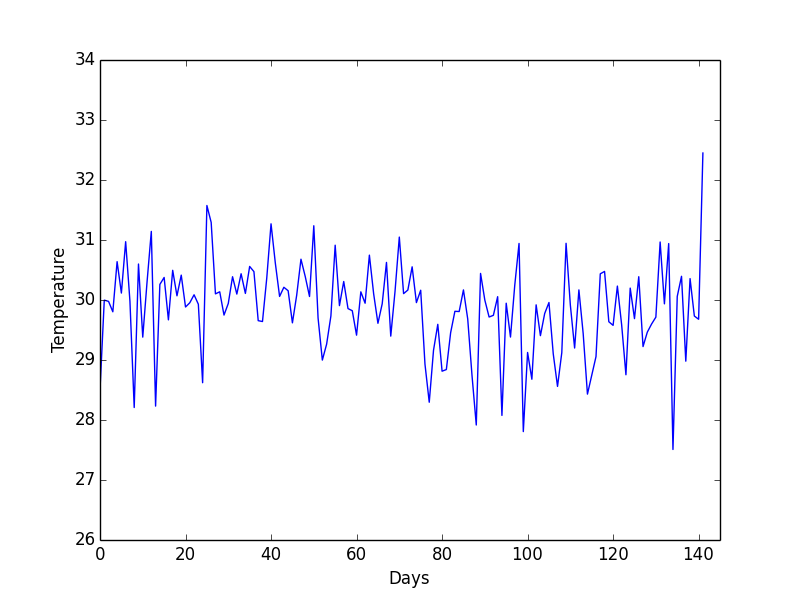
\includegraphics[width=\textwidth]{img/graphs/15-airtemp-1}
        \caption{S15}
        \label{fig:s15AT}
    \end{subfigure}
    ~ %add desired spacing between images, e. g. ~, \quad, \qquad, \hfill etc. 
      %(or a blank line to force the subfigure onto a new line)
    \begin{subfigure}[b]{0.30\textwidth}
        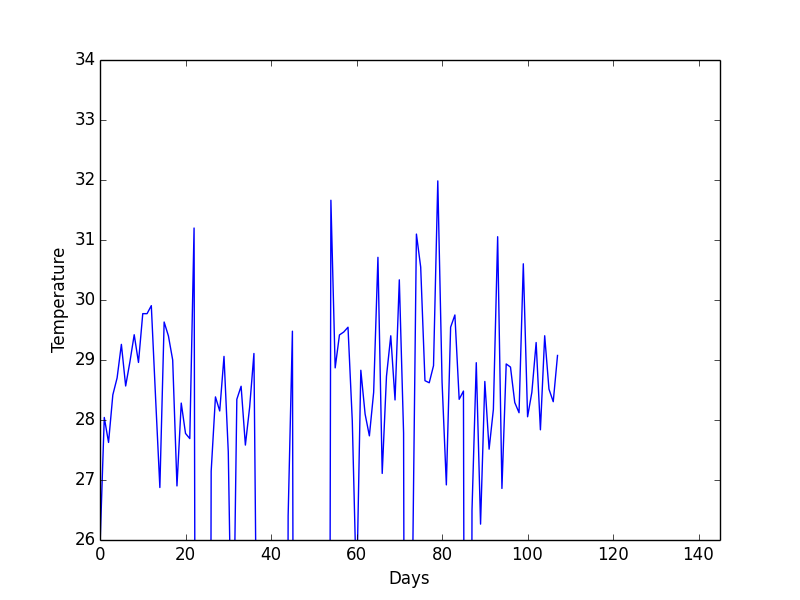
\includegraphics[width=\textwidth]{img/graphs/16-airtemp-1}
        \caption{S16}
        \label{fig:s16AT}
    \end{subfigure}
    ~ %add desired spacing between images, e. g. ~, \quad, \qquad, \hfill etc. 
      %(or a blank line to force the subfigure onto a new line)
    \begin{subfigure}[b]{0.2\textwidth}
        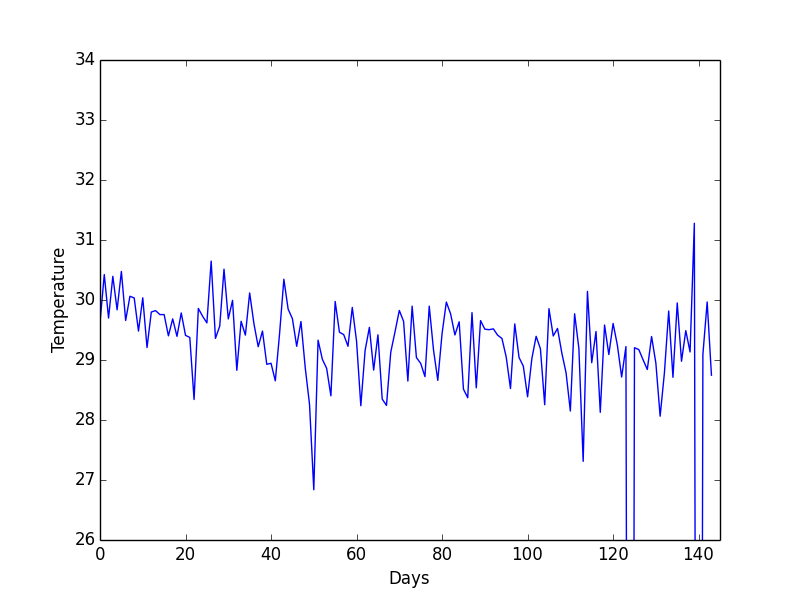
\includegraphics[width=\textwidth]{img/graphs/17-airtemp-1}
        \caption{S17}
        \label{fig:s17AT}
    \end{subfigure}
    ~ %add desired spacing between images, e. g. ~, \quad, \qquad, \hfill etc. 
      %(or a blank line to force the subfigure onto a new line)
    \begin{subfigure}[b]{0.2\textwidth}
        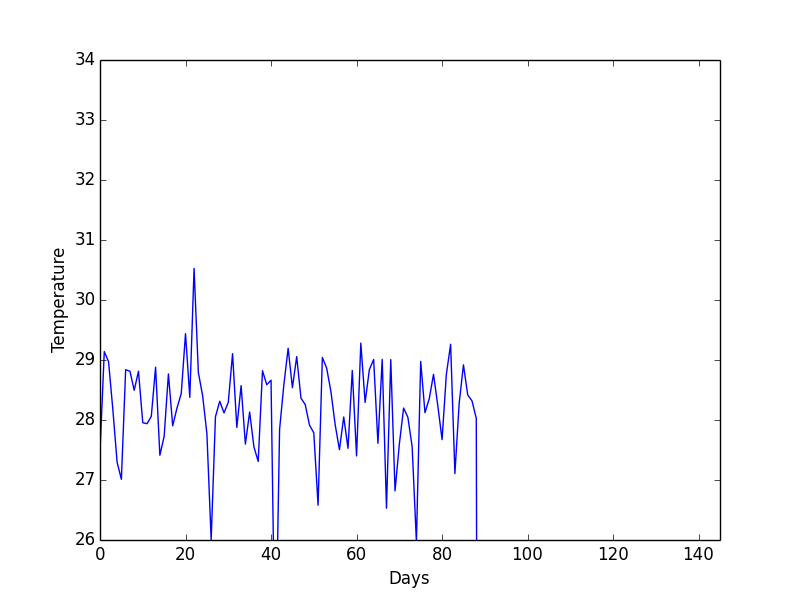
\includegraphics[width=\textwidth]{img/graphs/18-airtemp-1}
        \caption{S18}
        \label{fig:s18AT}
    \end{subfigure}
    ~ %add desired spacing between images, e. g. ~, \quad, \qquad, \hfill etc. 
      %(or a blank line to force the subfigure onto a new line)
    \begin{subfigure}[b]{0.2\textwidth}
        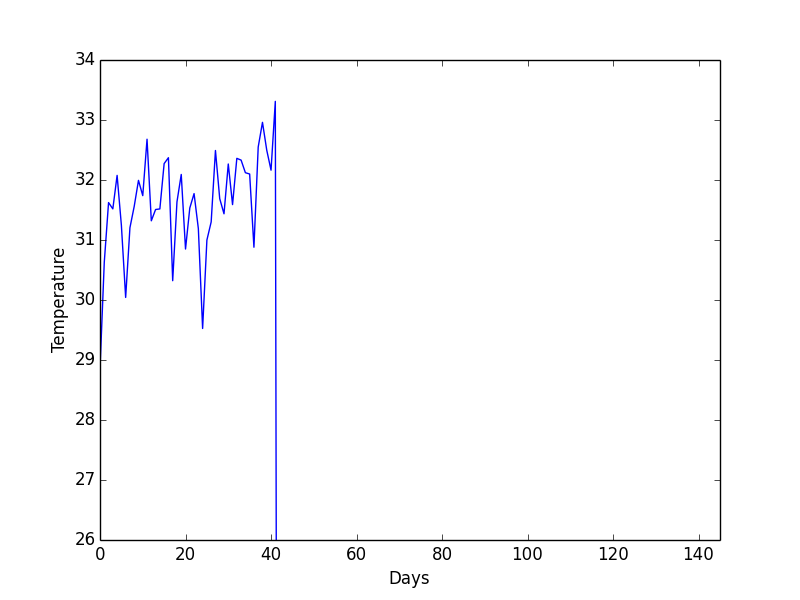
\includegraphics[width=\textwidth]{img/graphs/19-airtemp-1}
        \caption{S19}
        \label{fig:s19AT}
    \end{subfigure}
    ~ %add desired spacing between images, e. g. ~, \quad, \qquad, \hfill etc. 
      %(or a blank line to force the subfigure onto a new line)
    \begin{subfigure}[b]{0.2\textwidth}
        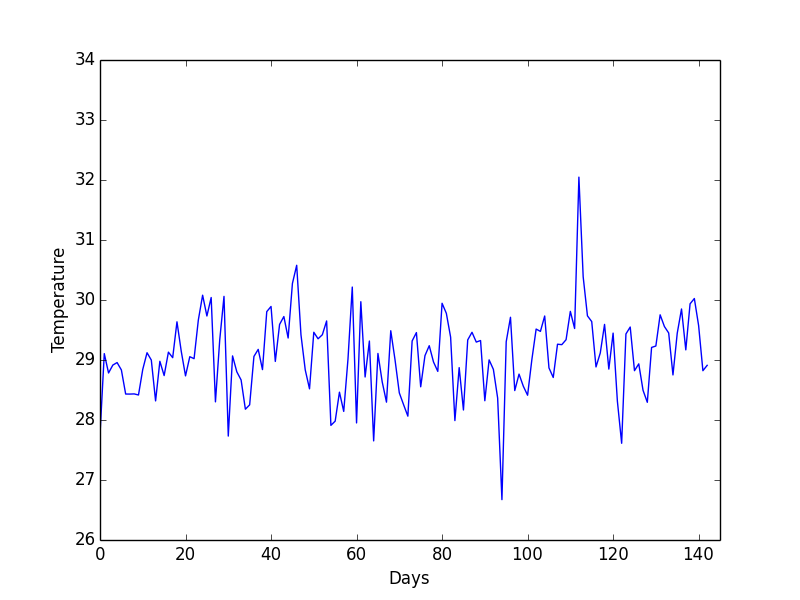
\includegraphics[width=\textwidth]{img/graphs/20-airtemp-1}
        \caption{S20}
        \label{fig:s20AT}
    \end{subfigure}
    \caption{Average air temperature on daily basis from beginning through March, 2016}
    \label{fig:avgAirTemp1}
\end{figure}


\begin{table}[H]
\center
\begin{footnotesize}
	\begin{tabular}{| c | c | c | c | c | c | c | c | c | c |}
	\hline
	\textbf{S\#} & \textbf{November} & \textbf{December} & \textbf{January} & \textbf{February} & \textbf{March} \\
	
	\hline
	S11 & 76.76 & 78.21 & 76.26 & 78.29 & 77.58\\
	\hline
	S12 & 73.47 & 74.24 & 75.25 & 70.33 & 71.91\\
	\hline
	S13 & 72.57 & 74.86 & 74.32 & 75.27 & 72.61\\
	\hline
	S14 & 78.44 & 76.30 & 77.65 & 77.30 & 78.06\\
	\hline
	S15 & 77.82 & 73.56 & 75.18 & 75.20 & 74.92\\
	\hline
	S16 & - & 72.89 & 72.80 & 74.31 & 72.59\\
	\hline
	S17 & 75.27 & 78.08 & 77.32 & 79.48 & 77.61\\
	\hline
	S18 & 80.88 & 82.15 & 86.23 & 79.48 & - \\
	\hline
	S19 & 87.41 & 83.89 & - & - & -\\
	\hline
	S20 & 74.19 & 72.02 & 73.81 & 79.56 & 76.75\\
	\hline
	\end{tabular}
	\caption{Average heartrate per month from beginning to March 31, 2016 - smartwatch.}
	\label{tab:heartrateWatch}
\end{footnotesize}
\end{table}

\begin{figure}[H]
    \centering
    \begin{subfigure}[b]{0.30\textwidth}
        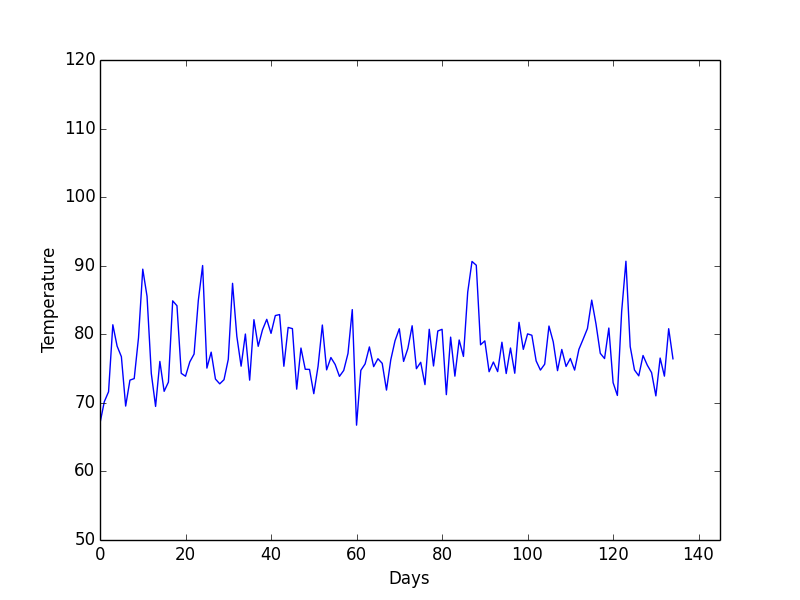
\includegraphics[width=\textwidth]{img/graphs/11-heartrate-1}
        \caption{S11}
        \label{fig:s11HT}
    \end{subfigure}
    ~ %add desired spacing between images, e. g. ~, \quad, \qquad, \hfill etc. 
      %(or a blank line to force the subfigure onto a new line)
    \begin{subfigure}[b]{0.30\textwidth}
        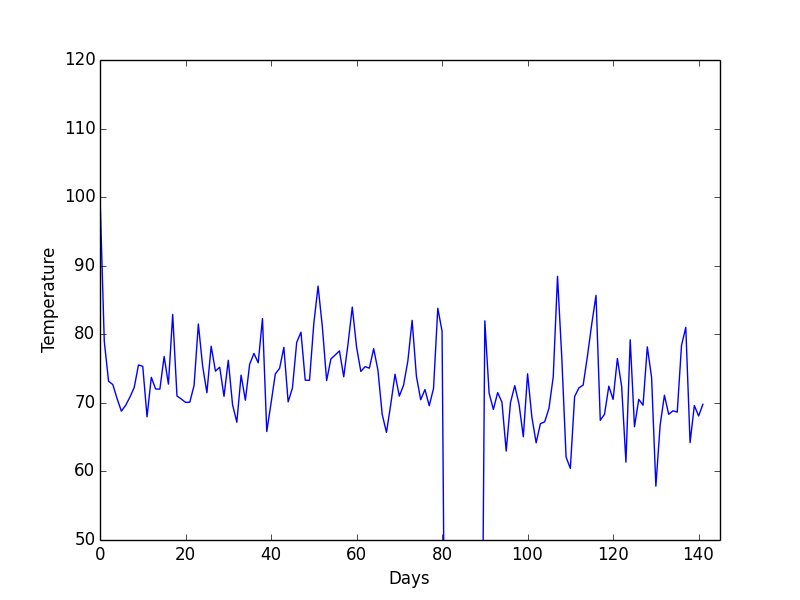
\includegraphics[width=\textwidth]{img/graphs/12-heartrate-1}
        \caption{S12}
        \label{fig:s12HT}
    \end{subfigure}
    ~ %add desired spacing between images, e. g. ~, \quad, \qquad, \hfill etc. 
      %(or a blank line to force the subfigure onto a new line)
    \begin{subfigure}[b]{0.30\textwidth}
        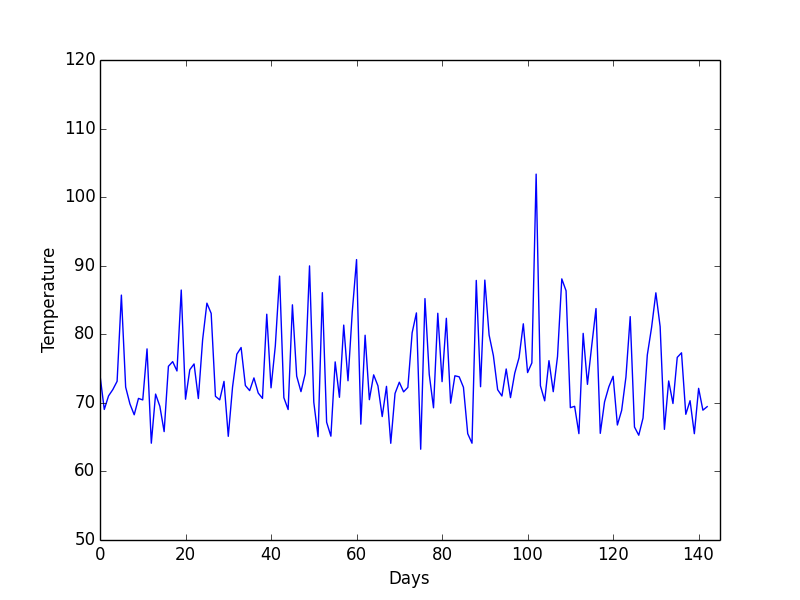
\includegraphics[width=\textwidth]{img/graphs/13-heartrate-1}
        \caption{S13}
        \label{fig:s13HT}
    \end{subfigure}
    ~ %add desired spacing between images, e. g. ~, \quad, \qquad, \hfill etc. 
      %(or a blank line to force the subfigure onto a new line)
    \begin{subfigure}[b]{0.30\textwidth}
        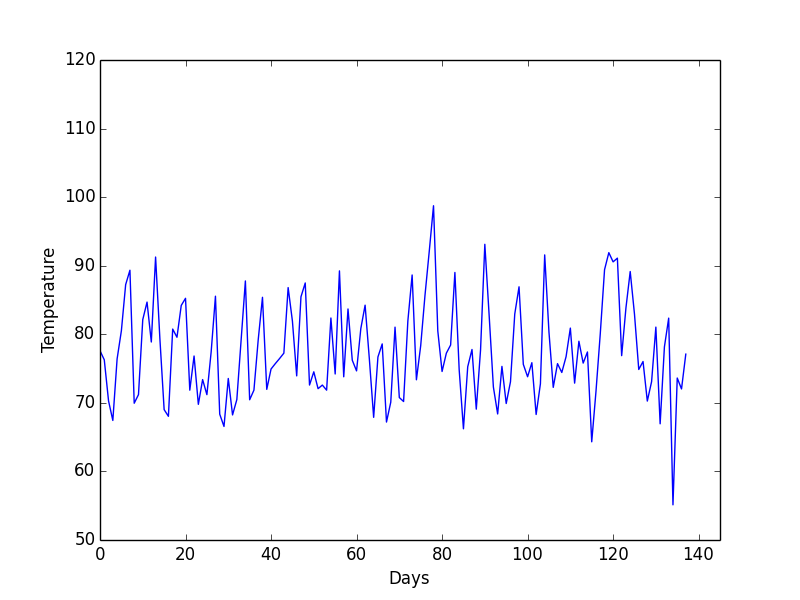
\includegraphics[width=\textwidth]{img/graphs/14-heartrate-1}
        \caption{S14}
        \label{fig:s14HT}
    \end{subfigure}
    ~ %add desired spacing between images, e. g. ~, \quad, \qquad, \hfill etc. 
      %(or a blank line to force the subfigure onto a new line)
    \begin{subfigure}[b]{0.30\textwidth}
        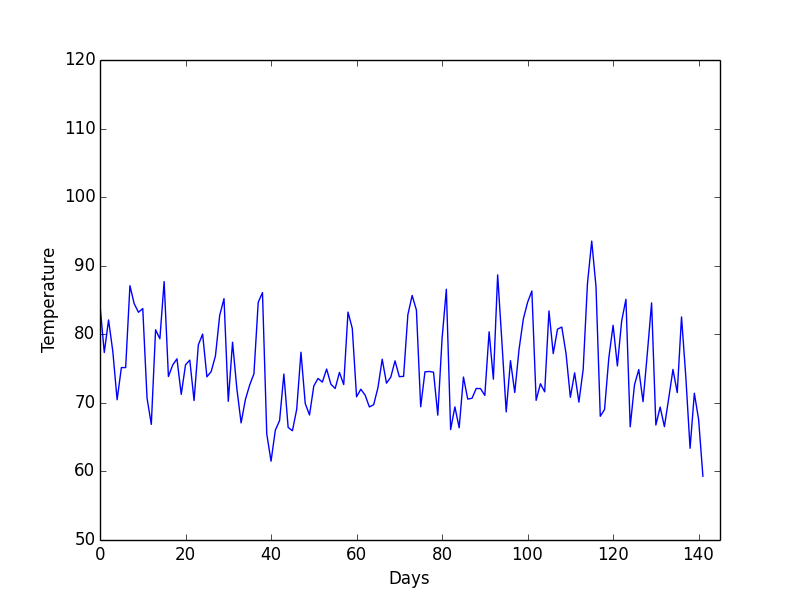
\includegraphics[width=\textwidth]{img/graphs/15-heartrate-1}
        \caption{S15}
        \label{fig:s15HT}
    \end{subfigure}
    ~ %add desired spacing between images, e. g. ~, \quad, \qquad, \hfill etc. 
      %(or a blank line to force the subfigure onto a new line)
    \begin{subfigure}[b]{0.30\textwidth}
        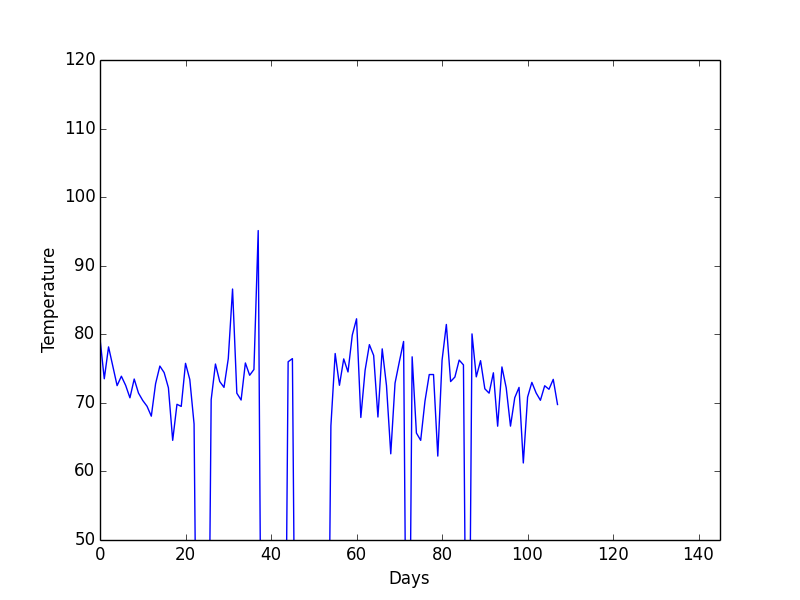
\includegraphics[width=\textwidth]{img/graphs/16-heartrate-1}
        \caption{S16}
        \label{fig:s16HT}
    \end{subfigure}
    ~ %add desired spacing between images, e. g. ~, \quad, \qquad, \hfill etc. 
      %(or a blank line to force the subfigure onto a new line)
    \begin{subfigure}[b]{0.2\textwidth}
        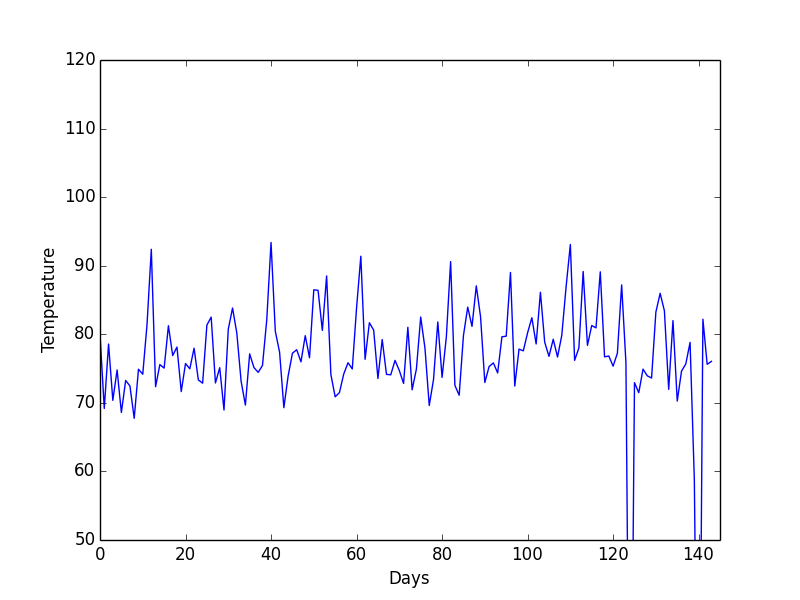
\includegraphics[width=\textwidth]{img/graphs/17-heartrate-1}
        \caption{S17}
        \label{fig:s17HT}
    \end{subfigure}
    ~ %add desired spacing between images, e. g. ~, \quad, \qquad, \hfill etc. 
      %(or a blank line to force the subfigure onto a new line)
    \begin{subfigure}[b]{0.2\textwidth}
        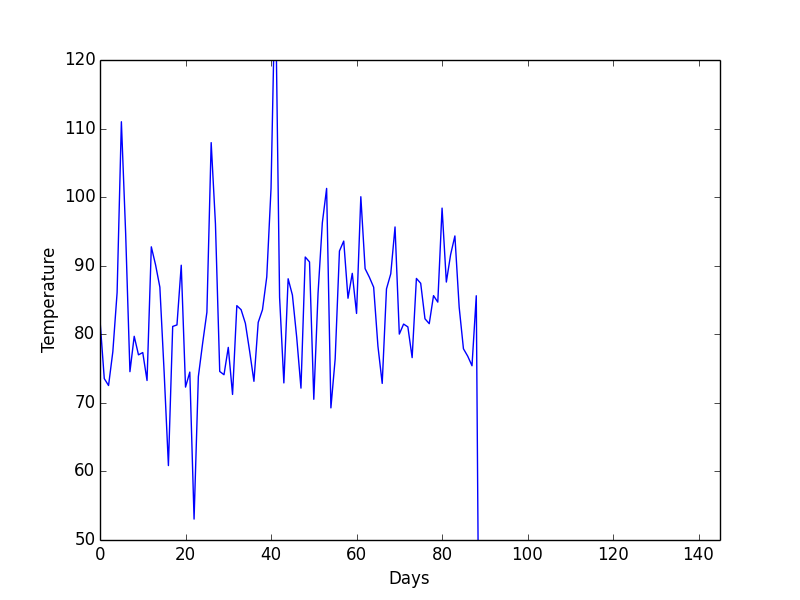
\includegraphics[width=\textwidth]{img/graphs/18-heartrate-1}
        \caption{S18}
        \label{fig:s18HT}
    \end{subfigure}
    ~ %add desired spacing between images, e. g. ~, \quad, \qquad, \hfill etc. 
      %(or a blank line to force the subfigure onto a new line)
    \begin{subfigure}[b]{0.2\textwidth}
        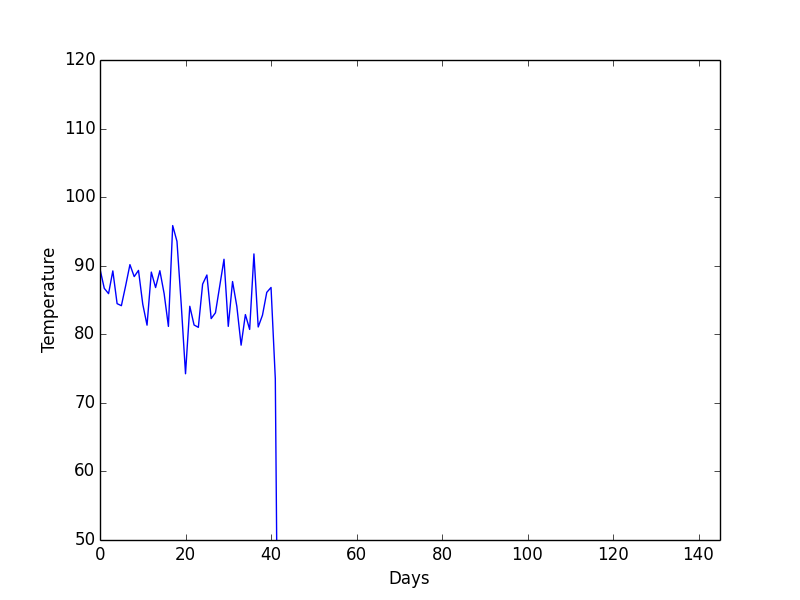
\includegraphics[width=\textwidth]{img/graphs/19-heartrate-1}
        \caption{S19}
        \label{fig:s19HT}
    \end{subfigure}
    ~ %add desired spacing between images, e. g. ~, \quad, \qquad, \hfill etc. 
      %(or a blank line to force the subfigure onto a new line)
    \begin{subfigure}[b]{0.2\textwidth}
        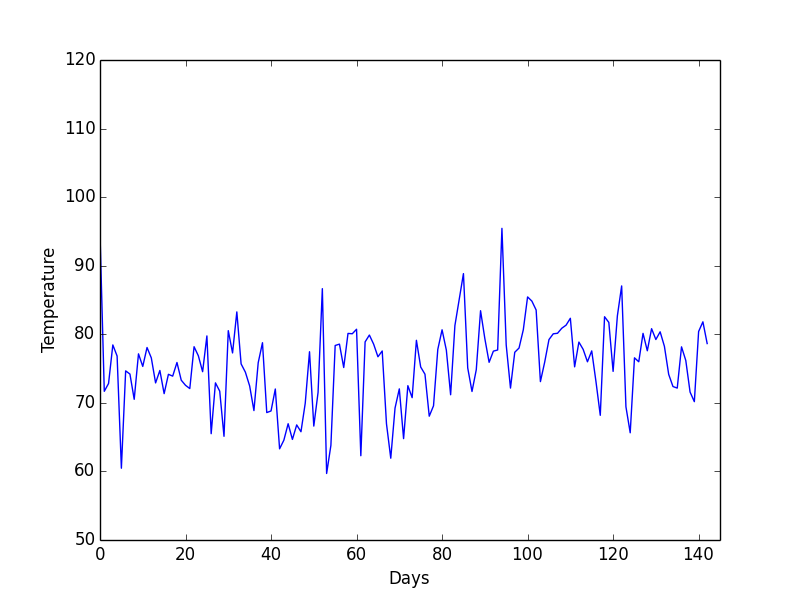
\includegraphics[width=\textwidth]{img/graphs/20-heartrate-1}
        \caption{S20}
        \label{fig:s20HT}
    \end{subfigure}
    \caption{Average heart rate on daily basis from beginning through March, 2016}
    \label{fig:avgheartrate}
\end{figure}


\begin{table}[H]
\center
\begin{footnotesize}
	\begin{tabular}{| c | c | c | c | c | c | c | c | c | c |}
	\hline
	\textbf{S\#} & \textbf{November} & \textbf{December} & \textbf{January} & \textbf{February} & \textbf{March} \\
	
	\hline
	S11 & 5736 & 6840 & 6610 & 8205 & 7512\\
	\hline
	S12 & 4489 & 3899 & 3733 & 2360 & 3488\\
	\hline
	S13 & 3944 & 4252 & 3470 & 4086 & 4436\\
	\hline
	S14 & 4539 & 3970 & 3263 & 4564 & 4284\\
	\hline
	S15 & 4531 & 4179 & 4726 & 4983 & 6151\\
	\hline
	S16 & - & 3445 & 2180 & 2723 & 3442\\
	\hline
	S17 & 7254 & 8065 & 9525 & 8446 & 8221\\
	\hline
	S18 & 7450 & 7200 & 7663 & 5128 & - \\
	\hline
	S19 & 6117 & 2512 & - & - & -\\
	\hline
	S20 & 7382 & 3810 & 3698 & 5755 & 5153\\
	\hline
	\end{tabular}
	\caption{Average steps per day in each month from beginning to March 31, 2016 - smartwatch.}
	\label{tab:stepsrateWatch}
\end{footnotesize}
\end{table}

\begin{figure}[H]
    \centering
    \begin{subfigure}[b]{0.30\textwidth}
        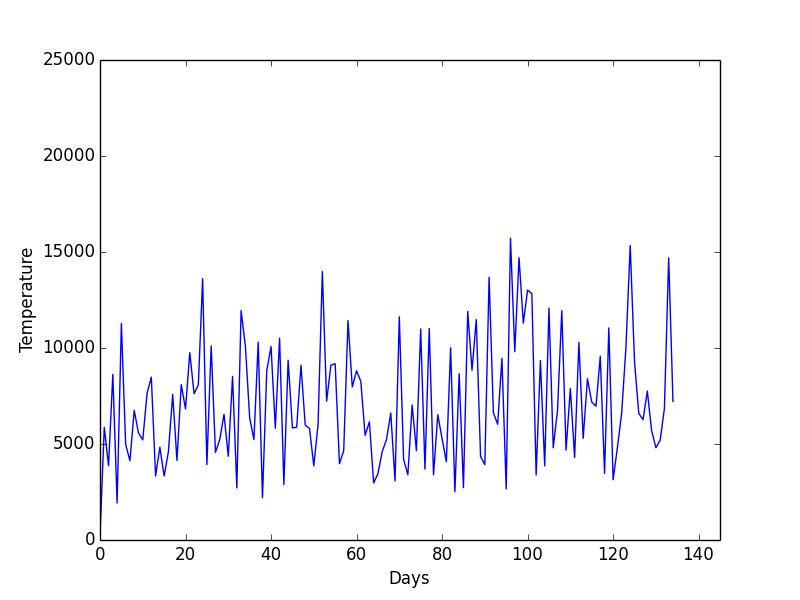
\includegraphics[width=\textwidth]{img/graphs/11-steps-1}
        \caption{S11}
        \label{fig:s11Steps}
    \end{subfigure}
    ~ %add desired spacing between images, e. g. ~, \quad, \qquad, \hfill etc. 
      %(or a blank line to force the subfigure onto a new line)
    \begin{subfigure}[b]{0.30\textwidth}
        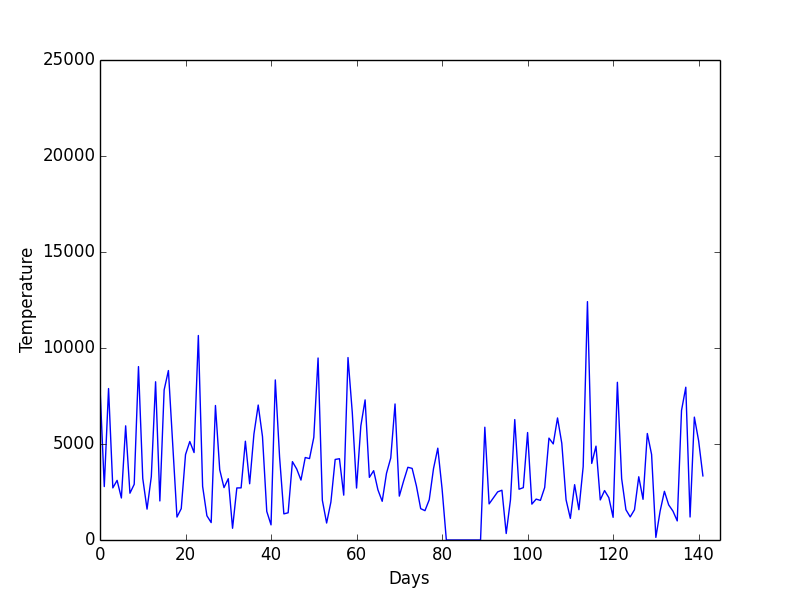
\includegraphics[width=\textwidth]{img/graphs/12-steps-1}
        \caption{S12}
        \label{fig:s12Steps}
    \end{subfigure}
    ~ %add desired spacing between images, e. g. ~, \quad, \qquad, \hfill etc. 
      %(or a blank line to force the subfigure onto a new line)
    \begin{subfigure}[b]{0.30\textwidth}
        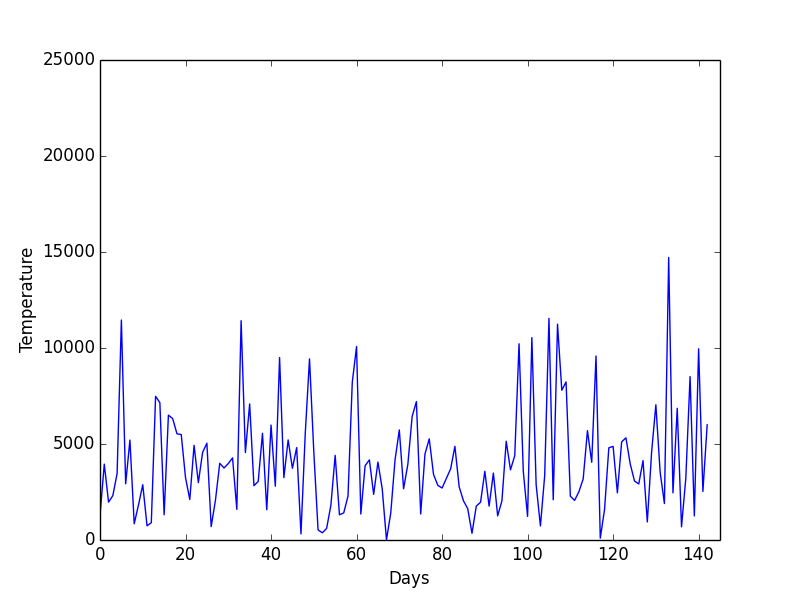
\includegraphics[width=\textwidth]{img/graphs/13-steps-1}
        \caption{S13}
        \label{fig:s13Steps}
    \end{subfigure}
    ~ %add desired spacing between images, e. g. ~, \quad, \qquad, \hfill etc. 
      %(or a blank line to force the subfigure onto a new line)
    \begin{subfigure}[b]{0.30\textwidth}
        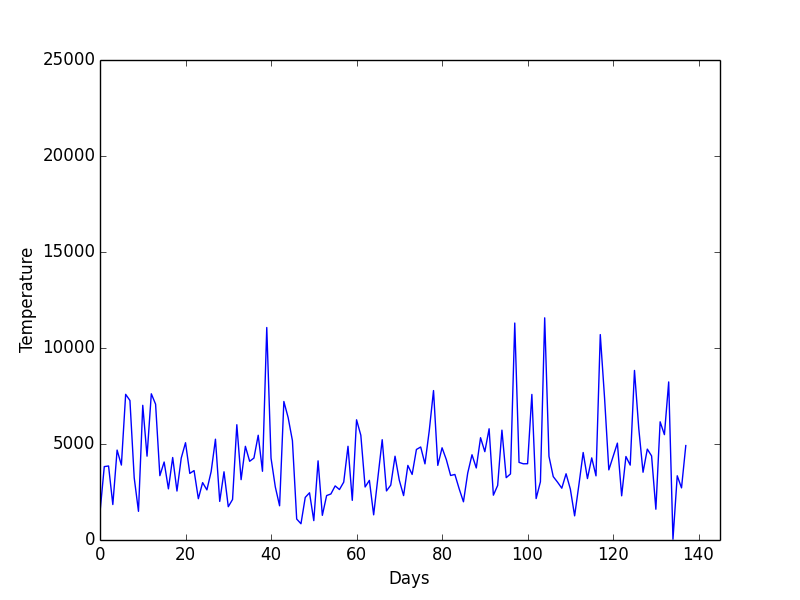
\includegraphics[width=\textwidth]{img/graphs/14-steps-1}
        \caption{S14}
        \label{fig:s14Steps}
    \end{subfigure}
    ~ %add desired spacing between images, e. g. ~, \quad, \qquad, \hfill etc. 
      %(or a blank line to force the subfigure onto a new line)
    \begin{subfigure}[b]{0.30\textwidth}
        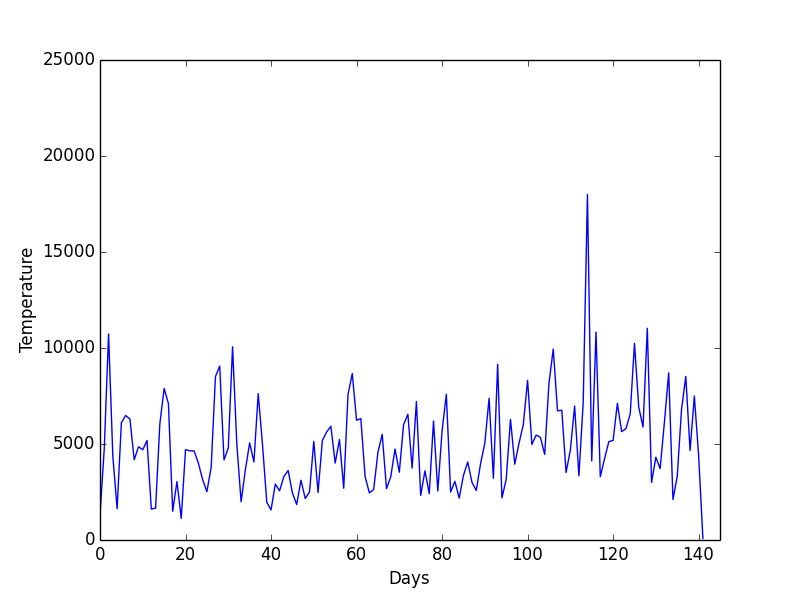
\includegraphics[width=\textwidth]{img/graphs/15-steps-1}
        \caption{S15}
        \label{fig:s15Steps}
    \end{subfigure}
    ~ %add desired spacing between images, e. g. ~, \quad, \qquad, \hfill etc. 
      %(or a blank line to force the subfigure onto a new line)
    \begin{subfigure}[b]{0.30\textwidth}
        \includegraphics[width=\textwidth]{img/graphs/16-steps-1}
        \caption{S16}
        \label{fig:s16Steps}
    \end{subfigure}
    ~ %add desired spacing between images, e. g. ~, \quad, \qquad, \hfill etc. 
      %(or a blank line to force the subfigure onto a new line)
    \begin{subfigure}[b]{0.2\textwidth}
        \includegraphics[width=\textwidth]{img/graphs/17-steps-1}
        \caption{S17}
        \label{fig:s17Steps}
    \end{subfigure}
    ~ %add desired spacing between images, e. g. ~, \quad, \qquad, \hfill etc. 
      %(or a blank line to force the subfigure onto a new line)
    \begin{subfigure}[b]{0.2\textwidth}
        \includegraphics[width=\textwidth]{img/graphs/18-steps-1}
        \caption{S18}
        \label{fig:s18Steps}
    \end{subfigure}
    ~ %add desired spacing between images, e. g. ~, \quad, \qquad, \hfill etc. 
      %(or a blank line to force the subfigure onto a new line)
    \begin{subfigure}[b]{0.2\textwidth}
        \includegraphics[width=\textwidth]{img/graphs/19-steps-1}
        \caption{S19}
        \label{fig:s19Step}
    \end{subfigure}
    ~ %add desired spacing between images, e. g. ~, \quad, \qquad, \hfill etc. 
      %(or a blank line to force the subfigure onto a new line)
    \begin{subfigure}[b]{0.2\textwidth}
        \includegraphics[width=\textwidth]{img/graphs/20-steps-1}
        \caption{S20}
        \label{fig:s20Step}
    \end{subfigure}
    \caption{Average steps on daily basis from beginning through March}
    \label{fig:avgsteps1}
\end{figure}


\begin{table}[H]
\center
\begin{footnotesize}
	\begin{tabular}{| c | c | c | c | c | c | c | c | c | c |}
	\hline
	\textbf{S\#} & \textbf{November} & \textbf{December} & \textbf{January} & \textbf{February} & \textbf{March} \\
	
	\hline
	S11 & 1.73 & 1.77 & 1.79 & 1.84 & 1.82\\
	\hline
	S12 & 1.39 & 1.40 & 1.58 & 1.43 & 1.50\\
	\hline
	S13 & 1.75 & 1.89 & 2.01 & 2.06 & 1.98\\
	\hline
	S14 & 3.42 & 3.34 & 3.20 & 3.28 & 3.18\\
	\hline
	S15 & 1.58 & 1.66 & 1.71 & 1.75 & 1.89\\
	\hline
	S16 & - & 1.76 & 1.63 & 1.59 & 1.72\\
	\hline
	S17 & 1.75 & 1.85 & 1.88 & 1.91 & 1.84\\
	\hline
	S18 & 2.31 & 2.43 & 3.01 & 2.62 & - \\
	\hline
	S19 & 1.54 & 1.21 & - & - & -\\
	\hline
	S20 & 1.42 & 1.32 & 1.47 & 1.53 & 1.46\\
	\hline
	\end{tabular}
	\caption{Average GSR per month from beginning to March 31, 2016 - smartwatch.}
	\label{tab:GSRWatch}
\end{footnotesize}
\end{table}

\begin{figure}[H]
    \centering
    \begin{subfigure}[b]{0.30\textwidth}
        \includegraphics[width=\textwidth]{img/graphs/11-gsr-1}
        \caption{S11}
        \label{fig:s11GSR}
    \end{subfigure}
    ~ %add desired spacing between images, e. g. ~, \quad, \qquad, \hfill etc. 
      %(or a blank line to force the subfigure onto a new line)
    \begin{subfigure}[b]{0.30\textwidth}
        \includegraphics[width=\textwidth]{img/graphs/12-gsr-1}
        \caption{S12}
        \label{fig:s12GSR}
    \end{subfigure}
    ~ %add desired spacing between images, e. g. ~, \quad, \qquad, \hfill etc. 
      %(or a blank line to force the subfigure onto a new line)
    \begin{subfigure}[b]{0.30\textwidth}
        \includegraphics[width=\textwidth]{img/graphs/13-gsr-1}
        \caption{S13}
        \label{fig:s13GSR}
    \end{subfigure}
    ~ %add desired spacing between images, e. g. ~, \quad, \qquad, \hfill etc. 
      %(or a blank line to force the subfigure onto a new line)
    \begin{subfigure}[b]{0.30\textwidth}
        \includegraphics[width=\textwidth]{img/graphs/14-gsr-1}
        \caption{S14}
        \label{fig:s14GSR}
    \end{subfigure}
    ~ %add desired spacing between images, e. g. ~, \quad, \qquad, \hfill etc. 
      %(or a blank line to force the subfigure onto a new line)
    \begin{subfigure}[b]{0.30\textwidth}
        \includegraphics[width=\textwidth]{img/graphs/15-gsr-1}
        \caption{S15}
        \label{fig:s15GSR}
    \end{subfigure}
    ~ %add desired spacing between images, e. g. ~, \quad, \qquad, \hfill etc. 
      %(or a blank line to force the subfigure onto a new line)
    \begin{subfigure}[b]{0.30\textwidth}
        \includegraphics[width=\textwidth]{img/graphs/16-gsr-1}
        \caption{S16}
        \label{fig:s16GSR}
    \end{subfigure}
    ~ %add desired spacing between images, e. g. ~, \quad, \qquad, \hfill etc. 
      %(or a blank line to force the subfigure onto a new line)
    \begin{subfigure}[b]{0.2\textwidth}
        \includegraphics[width=\textwidth]{img/graphs/17-gsr-1}
        \caption{S17}
        \label{fig:s17GSR}
    \end{subfigure}
    ~ %add desired spacing between images, e. g. ~, \quad, \qquad, \hfill etc. 
      %(or a blank line to force the subfigure onto a new line)
    \begin{subfigure}[b]{0.2\textwidth}
        \includegraphics[width=\textwidth]{img/graphs/18-gsr-1}
        \caption{S18}
        \label{fig:s18GSR}
    \end{subfigure}
    ~ %add desired spacing between images, e. g. ~, \quad, \qquad, \hfill etc. 
      %(or a blank line to force the subfigure onto a new line)
    \begin{subfigure}[b]{0.2\textwidth}
        \includegraphics[width=\textwidth]{img/graphs/19-gsr-1}
        \caption{S19}
        \label{fig:s19GSR}
    \end{subfigure}
    ~ %add desired spacing between images, e. g. ~, \quad, \qquad, \hfill etc. 
      %(or a blank line to force the subfigure onto a new line)
    \begin{subfigure}[b]{0.2\textwidth}
        \includegraphics[width=\textwidth]{img/graphs/20-gsr-1}
        \caption{S20}
        \label{fig:s20GSR}
    \end{subfigure}
    \caption{Average GSR on daily basis from beginning through March, 2016}
    \label{fig:avgGSR}
\end{figure}

\begin{table}[H]
\center
\begin{footnotesize}
	\begin{tabular}{| c | c | c | c | c | c | c | c | c | c |}
	\hline
	\textbf{S\#} & \textbf{November} & \textbf{December} & \textbf{January} & \textbf{February} & \textbf{March} \\
	
	\hline
	S11 & 2350 & 2549 & 2570 & 2646 & 2611\\
	\hline
	S12 & 1935 & 1980 & 2179 & 1614 & 2136\\
	\hline
	S13 & 2452 & 2703 & 2899 & 2962 & 2842\\
	\hline
	S14 & 4703 & 4802 & 4608 & 4716 & 4563\\
	\hline
	S15 & 2188 & 2382 & 2458 & 2486 & 2617\\
	\hline
	S16 & - & 2447 & 1764 & 1948 & 2434\\
	\hline
	S17 & 2445 & 2662 & 2705 & 2752 & 2543\\
	\hline
	S18 & 3220 & 3502 & 4335 & 2905 & - \\
	\hline
	S19 & 2140 & 1747 & - & - & -\\
	\hline
	S20 & 1995 & 1901 & 2118 & 2207 & 2093\\
	\hline
	\end{tabular}
	\caption{Average calories per month from beginning to March 31, 2016 - smartwatch.}
	\label{tab:caloriesWatch}
\end{footnotesize}
\end{table}

\begin{figure}[H]
    \centering
    \begin{subfigure}[b]{0.30\textwidth}
        \includegraphics[width=\textwidth]{img/graphs/11-calories-1}
        \caption{S11}
        \label{fig:s11cal}
    \end{subfigure}
    ~ %add desired spacing between images, e. g. ~, \quad, \qquad, \hfill etc. 
      %(or a blank line to force the subfigure onto a new line)
    \begin{subfigure}[b]{0.30\textwidth}
        \includegraphics[width=\textwidth]{img/graphs/12-calories-1}
        \caption{S12}
        \label{fig:s12cal}
    \end{subfigure}
    ~ %add desired spacing between images, e. g. ~, \quad, \qquad, \hfill etc. 
      %(or a blank line to force the subfigure onto a new line)
    \begin{subfigure}[b]{0.30\textwidth}
        \includegraphics[width=\textwidth]{img/graphs/13-calories-1}
        \caption{S13}
        \label{fig:s13cal}
    \end{subfigure}
    ~ %add desired spacing between images, e. g. ~, \quad, \qquad, \hfill etc. 
      %(or a blank line to force the subfigure onto a new line)
    \begin{subfigure}[b]{0.30\textwidth}
        \includegraphics[width=\textwidth]{img/graphs/14-calories-1}
        \caption{S14}
        \label{fig:s14cal}
    \end{subfigure}
    ~ %add desired spacing between images, e. g. ~, \quad, \qquad, \hfill etc. 
      %(or a blank line to force the subfigure onto a new line)
    \begin{subfigure}[b]{0.30\textwidth}
        \includegraphics[width=\textwidth]{img/graphs/15-calories-1}
        \caption{S15}
        \label{fig:s15cal}
    \end{subfigure}
    ~ %add desired spacing between images, e. g. ~, \quad, \qquad, \hfill etc. 
      %(or a blank line to force the subfigure onto a new line)
    \begin{subfigure}[b]{0.30\textwidth}
        \includegraphics[width=\textwidth]{img/graphs/16-calories-1}
        \caption{S16}
        \label{fig:s16cal}
    \end{subfigure}
    ~ %add desired spacing between images, e. g. ~, \quad, \qquad, \hfill etc. 
      %(or a blank line to force the subfigure onto a new line)
    \begin{subfigure}[b]{0.2\textwidth}
        \includegraphics[width=\textwidth]{img/graphs/17-calories-1}
        \caption{S17}
        \label{fig:s17cal}
    \end{subfigure}
    ~ %add desired spacing between images, e. g. ~, \quad, \qquad, \hfill etc. 
      %(or a blank line to force the subfigure onto a new line)
    \begin{subfigure}[b]{0.2\textwidth}
        \includegraphics[width=\textwidth]{img/graphs/18-calories-1}
        \caption{S18}
        \label{fig:s18cal}
    \end{subfigure}
    ~ %add desired spacing between images, e. g. ~, \quad, \qquad, \hfill etc. 
      %(or a blank line to force the subfigure onto a new line)
    \begin{subfigure}[b]{0.2\textwidth}
        \includegraphics[width=\textwidth]{img/graphs/19-calories-1}
        \caption{S19}
        \label{fig:s19cal}
    \end{subfigure}
    ~ %add desired spacing between images, e. g. ~, \quad, \qquad, \hfill etc. 
      %(or a blank line to force the subfigure onto a new line)
    \begin{subfigure}[b]{0.2\textwidth}
        \includegraphics[width=\textwidth]{img/graphs/20-calories-1}
        \caption{S20}
        \label{fig:s20cal}
    \end{subfigure}
    \caption{Average Calories on daily basis from beginning through March, 2016}
    \label{fig:avgCal}
\end{figure}

NOW YOU NEED TO MAKE THE SAME TABLES FOR THE PHONE DATA:
As seen in Table \ref{tab:ping} we work with 7 different file types that contains all our data collected via the smartphones. Below in Table \ref{tab:totalMinutesPhone} is listed how many minutes with any kind of data the files contain. As in Table \ref{tab:totalMinutesWatch}, Table \ref{tab:totalMinutesPhone} does not difference between what kind of data the files contain, only if there is data in them. 

\begin{table}[H]
\center
\begin{footnotesize}
	\begin{tabular}{| c || c | c | c | c | c | c | c | c | c | c |}
	\hline
	\textbf{S\#} & \textbf{User} & \textbf{Activity} & \textbf{Applications} & \textbf{CellIds} & \textbf{Touches} & \textbf{User} & \textbf{User}\\
	
	& \textbf{Precense} & \textbf{Serv} & \textbf{Used} & \textbf{Service} & \textbf{Buffered} & \textbf{Presence} &\textbf{Light} \\
	
	& \textbf{Events} & \textbf{Service} & & & & \textbf{Activity} & \\
	\hline
	S11 & & & & & & &\\
	S12 & & & & & & &\\
	S13 & & & & & & &\\
	S14 & & & & & & &\\
	S15 & & & & & & &\\
	S16 & & & & & & &\\
	S17 & & & & & & &\\
	S18 & & & & & & &\\
	S19 & & & & & & &\\
	S20 & & & & & & &\\
	\hline
	\end{tabular}
	\caption{Days and nights with any kind of data from beginning to March 31, 2016 - smartphone.}
	\label{tab:totalMinutesPhone}
\end{footnotesize}
\end{table}

In table \ref{tab:daysNightsExp1Phone} a total number of days and nights with any kind of data is listed. The definition of days and nights for the smartphones is defined like this: \todo{FIND SOMETHING TO WRITE HERE}. ALSO WRITE SOMETHING ABOUT HOW YOU DEFINED WHEN A DAY/NIGHT IS VALID OR INVALID AND WHY!

\begin{table}[H]
\center
\begin{footnotesize}
	\begin{tabular}{| c | c | c || c | c | c | c | c | c | c | c |}
	\hline
	\textbf{S\#} & \textbf{Total} & \textbf{Total} & \textbf{Days} & \textbf{Nights} \\
	& \textbf{Days} & \textbf{Nights} & & \\
	\hline
	S11 & & & & \\
	S12 & & & & \\
	S13 & & & & \\
	S14 & & & & \\
	S15 & & & & \\
	S16 & & & & \\
	S17 & & & & \\
	S18 & & & & \\
	S19 & & & & \\
	S20 & & & & \\
	\hline
	\end{tabular}
	\caption{Days and nights with any kind of data from beginning to March 31, 2016 - smartphone.}
	\label{tab:daysNightsExp1Phone}
\end{footnotesize}
\end{table}


\subsubsection{Sleep Quantity Assessment}
\paragraph{Sleep Quantity Results}


\subsubsection{Sleep Quality Assessment}
\paragraph{Sleep Quality Results}




\newpage
\subsection{Experiment \#2}
\subsubsection{Sleep Quantity Assessment}
\paragraph{Sleep Quantity Results}



\subsubsection{Sleep Quality Assessment}
\paragraph{Sleep Quality Results}



\newpage
ALT HERUNDER ER RUBBISH
%%%%%%%%%%%%%%%%%%%%%%%%%%%%%%%%%%%%%%%%%%%%%%%%%%%%%%%%%%%%%%%
%%%%%%%%%%%%%%%%%%%%%%%%%%%%%%%%%%%%%%%%%%%%%%%%%%%%%%%%%%%%%%%
%%%%%%%%%%%%%%%%%%%%%%%%%%%%%%%%%%%%%%%%%%%%%%%%%%%%%%%%%%%%%%%
%%%%%%%%%%%%%%%%%%%%%%%%%%%%%%%%%%%%%%%%%%%%%%%%%%%%%%%%%%%%%%%
%%%%%%%%%%%%%%%%%%%%%%%%%%%%%%%%%%%%%%%%%%%%%%%%%%%%%%%%%%%%%%%
%%%%%%%%%%%%%%%%%%%%%%%%%%%%%%%%%%%%%%%%%%%%%%%%%%%%%%%%%%%%%%%
%%%%%%%%%%%%%%%%%%%%%%%%%%%%%%%%%%%%%%%%%%%%%%%%%%%%%%%%%%%%%%%
%%%%%%%%%%%%%%%%%%%%%%%%%%%%%%%%%%%%%%%%%%%%%%%%%%%%%%%%%%%%%%%
%%%%%%%%%%%%%%%%%%%%%%%%%%%%%%%%%%%%%%%%%%%%%%%%%%%%%%%%%%%%%%%
%%%%%%%%%%%%%%%%%%%%%%%%%%%%%%%%%%%%%%%%%%%%%%%%%%%%%%%%%%%%%%%
%\newpage	
%\section{Data collection}
%\subsection{Experiment \#1}
%\label{sec:experiment1}
%This chapter is about the participants and the data collected from November 2015 to end of March 2016. The quality of the data was investigated, and during this investigation interesting questions came up. From the DRM's and the initial survey it was seen that some participants worked out more than others, and it was researched if participants slept better or worse after a work out compared to other days and if the subjects who worked out in general slept better than the subjects who did not work out. Statistics was made to see if there was difference in sleep in weekdays and weekends/holidays. It was also investigated if exam periods influenced the sleep quantity and quality and if master students had different sleep patterns than bachelor students, and if being in a relationship seems to affect the sleeping patterns. \\
%\todo[inline]{these things should of course also be investigated for the second period and compared with the first one}






\subsubsection{Results}
Sleep statistics, phone usage stats (on/off/present). 


Algorithm\\

\textbf{MOVED FROM RELATED WORK:}
Looking at the data I have collected from the participants, it was clear that not only was the circadian rhythm important for participants sleep patterns, but the stages of the actual sleep are also important. 





\subsection{Experiment \# 2}
April to midt July - dataset for machinelearning (learn on dataset from midt November to March and then run on experiment 2 data for evaluation)\\

I also want to see if there is any difference in how long people sleep - my guess is, that people sleep lesser when it gets hotter and lighter outside. I would like to see if the data agrees on me on this. In better words - does the students circadian rhythm change when it gets warmer and lighter outside?

%The user experiment was running from November 2015 to June 2016 and included ten participants. The first four weeks for each participant was used to set up the smartphone and the BASIS watch. Also I met with each participant once a week for all four weeks to ask questions if any to the collected data, and to reconstruct a complete day for each of the four weeks. These four weeks is also referred to as the first stage or the first user experiment. \\

%After the four weeks each participant was told to wear the watch and use their phone just as they used to do, and if they did not hear from me, then they could assume, that everything was working fine. I still collected their data, but otherwise I did not had any interference with them. This part is the second stage of the experiment, and the last stage is what is referred to as the follow up experiment in Figure \ref{fig:timeline}. Once again I met with each participant once a week for four weeks, checking up on everything, reconstructing a total of four days and asked questions if any was needed. \\

%The design of the experiment and the participants is described in details in Section \ref{sec:design}, the results in Section \ref{sec:experiment}, and the analysis of the first stage of data is described in Section \ref{sec:analysis}. Further more, in Section \ref{subsubsec:pilot} there is a description of the pilot test of the watches used in the experiment. 


%THIS BELOW  IS ONLY SAVED FOR THE TABLE AGTIGT!!

%Something about QoL and Social Fabric ($\rightarrow$ initial idea of what to look for)\\

%\begin{table}[H]
%\center
%\begin{footnotesize}
%	\begin{tabular}{|p{0.4cm} |p{2cm} |p{2.5cm} |p{2cm} |p{2.1cm} |p{2.2cm} |p{1.8cm} |}
%	\hline
%	\textbf{\#} & \textbf{Goal} & \textbf{Input} & \textbf{Procedure} & \textbf{Output} & \textbf{\# People} & \textbf{Time}\\
%	\hline
%	\hline
%	\#4 & TBD & TBD & TBD & TBD & TBD & TBD \\
%	\hline
%	\#5 & TBD & TBD & TBD & TBD & TBD & TBD \\
%	\hline 
%	\end{tabular}
%	\caption{State of the art - data available}
%	\label{tab:mQoLSocialFabric}
%\end{footnotesize}
%\end{table}

\section{Discussion}
- Factors influencing the quality of data (what could go wrong and how did I manage?\\
- Limitations\\
- Technology used\\
- Human related factors (adherence)\\

In chapter 2 I ended a paragraph writing: ``giving people three highly complicated and individually diverse factors influencing and affecting our timing and quality of sleep: our circadian system, a homeostatic oscillator, and our social time.'' Now discuss what I found in my population with relation to these factors.

\section{Design Implications}
Provide design implications for a digital solution for mobilephones to help combat unhealthy behaviour in students sleeping patterns

\section{Conclusion}


\newpage
%\bibliographystyle{plainnat}
\bibliographystyle{unsrt}
\bibliography{bibliography}

\newpage
\appendix
\section{Entry Survey} \label{sec:survey}

%\includepdf[pages=1-9, pagecommand={}, scale=0.5]{survey.pdf}

\begin{figure}[H]
 \centering 
 \includepdf[pages=1,scale=0.9, pagecommand={}]{pdf/survey.pdf}
\end{figure}

\newpage
\begin{figure}[H]
 \centering 
 \includepdf[pages=2,scale=0.9, pagecommand={}]{pdf/survey.pdf}
\end{figure}

\newpage
\begin{figure}[H]
 \centering 
 \includepdf[pages=3,scale=0.9, pagecommand={}]{pdf/survey.pdf}
\end{figure}

\newpage
\begin{figure}[H]
 \centering 
 \includepdf[pages=4,scale=0.9, pagecommand={}]{pdf/survey.pdf}
\end{figure}

\newpage
\begin{figure}[H]
 \centering 
 \includepdf[pages=5,scale=0.9, pagecommand={}]{pdf/survey.pdf}
\end{figure}

\newpage
\begin{figure}[H]
 \centering 
 \includepdf[pages=6,scale=0.9, pagecommand={}]{pdf/survey.pdf}
\end{figure}

\newpage
\begin{figure}[H]
 \centering 
 \includepdf[pages=7,scale=0.9, pagecommand={}]{pdf/survey.pdf}
\end{figure}

\newpage
\begin{figure}[H]
 \centering 
 \includepdf[pages=8,scale=0.9, pagecommand={}]{pdf/survey.pdf}
\end{figure}

\newpage
\begin{figure}[H]
 \centering 
 \includepdf[pages=9,scale=0.9, pagecommand={}]{pdf/survey.pdf}
\end{figure}

\newpage
\begin{figure}[H]
 \centering 
 \includepdf[pages=10,scale=0.9, pagecommand={}]{pdf/survey.pdf}
\end{figure}

\newpage
\begin{figure}[H]
 \centering 
 \includepdf[pages=11,scale=0.9, pagecommand={}]{pdf/survey.pdf}
\end{figure}

\newpage
\section{Ping App V. 2 Data Files} \label{sec:ping}
\begin{figure}[H]
 \centering 
 \includepdf[pages=1,scale=0.9, pagecommand={}]{pdf/ping_v2_data_description.pdf}
\end{figure}

\newpage
\begin{figure}[H]
 \centering 
 \includepdf[pages=2,scale=0.9, pagecommand={}]{pdf/ping_v2_data_description.pdf}
\end{figure}

\newpage
\begin{figure}[H]
 \centering 
 \includepdf[pages=3,scale=0.9, pagecommand={}]{pdf/ping_v2_data_description.pdf}
\end{figure}

\newpage
\begin{figure}[H]
 \centering 
 \includepdf[pages=4,scale=0.9, pagecommand={}]{pdf/ping_v2_data_description.pdf}
\end{figure}

\newpage
\begin{figure}[H]
 \centering 
 \includepdf[pages=5,scale=0.9, pagecommand={}]{pdf/ping_v2_data_description.pdf}
\end{figure}

\newpage
\begin{figure}[H]
 \centering 
 \includepdf[pages=6,scale=0.9, pagecommand={}]{pdf/ping_v2_data_description.pdf}
\end{figure}

\newpage
\section{Subset of Basis Retriever Data} \label{sec:subset}
\begin{figure}[H]
 \centering 
 \includepdf[page=1,scale=0.9, pagecommand={}]{pdf/retriever}
\end{figure}



\newpage
\section{Labelling of DRM} \label{sec:drm}
\todo[inline]{Put in the labelling from all DRM's}


%\includepdf[pages=1-9, pagecommand={}, scale=0.5]{survey.pdf}



\end{document}